\documentclass[a4paper, % A4
	parskip, % Absätze durch Abstand statt Einrückung gekennzeichnet
	%draft, % überlange Zeilen werden nicht%markiert
	ngerman] % english, hyphenation etc.
	{scrreprt} % Report (KOMA-Script)

\usepackage[T1]{fontenc} % Font family encoding: 8 Bit
\usepackage[utf8]{inputenc} % Encoding in the created document: UTF-8
\usepackage{lmodern} % Font family
\usepackage[babel]{microtype} % Automatische Grauwertverbesserung
\usepackage[ngerman]{babel} % warning that option english is not loaded yet
    % when not declaring [USenglish] even though documentclass sets it globally
\usepackage{IEEEtrantools} % bibliography, quoting (\cite)

%Text wrapped around figures
\usepackage{wrapfig}

% Better tables
\usepackage{tabularx}
\newcolumntype{b}{X}
\newcolumntype{s}{>{\hsize=.5\hsize}X}

%Better quotes..
\usepackage{csquotes}

%Checkboxes
\usepackage{wasysym}

\usepackage{graphicx} % include images (\includegrafics)
\usepackage[section]{placeins} % place floating objects before a \FloatBarrier

\usepackage{framed} % frame paragraphs (\begin{framed})
\usepackage{geometry} % change margin for title page (\newgeometry,
	% \resetgeometry)
\usepackage{setspace} % change line spacing (\onehalfspacing)
\usepackage{pdflscape} % pages in landscape (\begin{landscape})
\usepackage{multicol} % multiple columns for a sector (\begin{multicols})

\usepackage{rotating} % begin{sidewaysfigure} end{..}

\usepackage{booktabs} % Professional looking tables (\toprule,% \midrule,
	% \bottomrule)
\usepackage{threeparttable} % table with notes (\tnote, \begin{tablenotes})
\usepackage{longtable}
\usepackage[table,xcdraw]{xcolor}

\usepackage[printonlyused, % show only used acronyms
		% withpage, % show pagenumber of first usage
	] % longform in footnote (instead of shortform)
	{acronym} % abbreviations  (\ac, \acs,\acl)
		% \begin{acronym})
		
\usepackage{pdfpages} % include PDFs (\includepdf)
\usepackage{listings} % codelistings (\lstnewenvironment)
\usepackage{float} % own floating objects (\newfloat, \floatname)

\usepackage{hyperref} % linking to refs and URLs (\ref, \url, \autoref,
% \nameref)
%rename the output for an \autoref{chap:XXX} from lowercase chapter to Chapter
% and also for Section and Subsection
\addto\extrasUSenglish{%
  \renewcommand{\chapterautorefname}{Chapter}% 
}
\addto\extrasUSenglish{%
  \renewcommand{\sectionautorefname}{Section}% 
}
\addto\extrasUSenglish{%
  \renewcommand{\subsectionautorefname}{Subsection}% 
}

\usepackage{scrhack} % \lstlistoflistings uses deprecated \float@listhead,
    % scrhack fixes this warning (redefines macros from other packages so they
    % work better with KOMAscript)


% global formatting
\onehalfspacing % 1.5x line spacing

\usepackage{color}

% colors for syntax highlighting
\definecolor{strings}{RGB}{42,0,255}
\definecolor{builtInTypes}{RGB}{127,0,85}
\definecolor{comments}{RGB}{63,127,95}

\lstdefinestyle{CPPeclipse}{
    basicstyle=\ttfamily,
    stringstyle=\color{strings},     
    keywordstyle=\color{builtInTypes} \bfseries,
    commentstyle=\color{comments},
    %emph={int,char,double,float,unsigned},
    %emphstyle={\color{blue}},
}

\definecolor{pblue}{rgb}{0.13,0.13,1}
\definecolor{pgreen}{rgb}{0,0.5,0}
\definecolor{pred}{rgb}{0.9,0,0}
\definecolor{pgrey}{rgb}{0.46,0.45,0.48}


\lstdefinestyle{JavaEclipse}{
    basicstyle=\ttfamily,
    commentstyle=\color{pgreen},
    keywordstyle=\color{pblue},
    stringstyle=\color{pred},
}

% Standard Listing
\lstset{
	aboveskip=1.5\baselineskip,      % space before listing
	breakatwhitespace=true,          % break only at whitespace
	breaklines=true,                 % sets automatic line breaking
	captionpos=b,                    % sets the caption-position to bottom
	extendedchars=true,              % lets you use non-ASCII characters; for 8-bits encodings only, does not work with UTF-8
	frame=single,                    % adds a frame around the code
	keepspaces=true,                 % keeps spaces in text, useful for keeping indentation of code (possibly needs columns=flexible)
	language=C++,                    % the language of the code, [11] indicates
	                                 % C++ 11syntax. other possible values:
	                                 %     ANSI, GNU, VISUAL ISO
	numbers=left,                    % where to put the line-numbers; possible values are (none, left, right)
	showspaces=false,                % show spaces everywhere adding particular underscores; it overrides 'showstringspaces'
	showstringspaces=false,          % underline spaces within strings only
	showtabs=false,                  % show tabs within strings adding particular underscores
	tabsize=3,                       % sets default tabsize in spaces
	style=CPPeclipse
}


\colorlet{punct}{red!60!black}
\definecolor{background}{HTML}{EEEEEE}
\definecolor{delim}{RGB}{20,105,176}
\colorlet{numb}{magenta!60!black}

\lstdefinelanguage{json}{
    stepnumber=1,
    breaklines=true,
    literate=
     *{0}{{{\color{numb}0}}}{1}
      {1}{{{\color{numb}1}}}{1}
      {2}{{{\color{numb}2}}}{1}
      {3}{{{\color{numb}3}}}{1}
      {4}{{{\color{numb}4}}}{1}
      {5}{{{\color{numb}5}}}{1}
      {6}{{{\color{numb}6}}}{1}
      {7}{{{\color{numb}7}}}{1}
      {8}{{{\color{numb}8}}}{1}
      {9}{{{\color{numb}9}}}{1}
      {:}{{{\color{punct}{:}}}}{1}
      {,}{{{\color{punct}{,}}}}{1}
      {\{}{{{\color{delim}{\{}}}}{1}
      {\}}{{{\color{delim}{\}}}}}{1}
      {[}{{{\color{delim}{[}}}}{1}
      {]}{{{\color{delim}{]}}}}{1},
}
% change the name from 'List of Listings' to something else
% \renewcommand{\lstlistlistingname}{Listingverzeichnis}
\newcommand{\code}[1]
	{\texttt{#1}}
\newcommand{\command}[1]
    {\textit{#1}}
\newcommand{\filepath}[1]
	{\texttt{#1}}
\newcommand*{\fullref}[1]
    {\hyperref[{#1}]{\autoref*{#1} \nameref*{#1} on page \pageref*{#1}}}
\newcommand{\linenumber}[1]
    {\textit{#1}}
\newcommand{\productname}[1]
	{\textit{#1}}
\newcommand{\tbd}[1]
    {{\color{red}<tbd> #1}}
\newfloat{listingfloat}{htb}{qcl}[chapter]
\floatname{listingfloat}{Listing}

% definiton of frequenlty used standard texts.
% Usage in text: \ecdt{} -> Eclipse CDT

\newcommand{\advisor}
	{Tobias Brunner}
\newcommand{\advisorprof}
	{Prof. Dr. Andreas Steffen}
\newcommand{\contraprof}
	{Prof. Dr. Josef Joller}
\newcommand{\expert}
	{Dr. Ralf Hauser}
\newcommand{\osag}
	{Open Systems AG }
\newcommand{\authors}
	{Jan Balmer, Theo Winter}
\newcommand{\esp}
	{\acs{ESP}}
\newcommand{\tool}
    {IPsec Diagnose Tool}
\newcommand{\entool}
    {IPsec Diagnosis Tool}
\newcommand{\ipsec}
    {\acs{IPsec}}
\newcommand{\place}
	{HSR---Hochschule für Technik Rapperswil \\ Institut für Internet-Technologien
	und -Anwendungen}
\newcommand{\product}
	{\productname{\ecdt{} IPSecDiagTool \pg{}}}
\newcommand{\timeperiod}
	{Frühjahrssemester 2015}
\newcommand{\titel}
	{IPSec Diagnose Tool}
\newcommand{\work}
	{Semester-/Bachelorarbeit }
 
\begin{document}

%Intro-Teil
% Following the template unter www.hsr.ch > HSR-intern > Bachelor-Studiengänge
% > Informatik > allgemeine Infos Diplom-, Bachelor- und Studienarbeiten.

\newgeometry{left=2.25cm, right=2.25cm, top=2.25cm, bottom=2.25cm} % new
% margins

\begin{titlepage}
%TODO: set logo position exactly.
\begin{center}
\begin{minipage}[t]{0.45\textwidth}
    
\includegraphics[width=\textwidth]{start/img/hsrLogo}
\end{minipage}
\hspace{\fill} % horizontal space
\begin{minipage}[t]{0.45\textwidth}
    \vspace{-2.56cm}
    
\includegraphics[width=\textwidth]{start/img/itaLogo} %TODO: more highres logo
\end{minipage}

\end{center}

\vspace{15ex} % vertical space
\begin{center}
	\Huge 
	\begin{framed}
		\textbf{\titel}
	\end{framed}
	
	\vspace{3ex}
	\textbf{\work}
	
	\vspace{1ex}
	\LARGE 
	\place
	
	\vspace{5ex}
	\begin{framed}
		\timeperiod
	\end{framed}
\end{center}

\vspace{11ex}
\begin{tabular}{ll} % Table
	Autoren:         		& \authors    	\\
	Betreuender Dozent:		& \advisorprof  	\\
	Betreuer:        		& \advisor    	\\
	Gegenleser:      		& \contraprof  	\\
	Experte:      			& \expert  		\\
	Industriepartner:      	& \osag  		\\
\end{tabular}

\end{titlepage}

\restoregeometry % reset page margins

% Der Abstract richtet sich an den Spezialisten auf dem entsprechenden Gebiet
% und beschreibt daher in erster Linie die (neuen, eigenen) Ergebnisse und
% Resultate der Arbeit. Es umfasst nie mehr als eine Seite, typisch sogar nur
% etwa 200 Worte (etwa 20 Zeilen). Es sind keine Bilder zu verwenden.

\chapter*{Abstract}\addcontentsline{toc}{chapter}{Abstract}

Paket Verluste und Fragmentierungsprobleme treten bei VPN Verbindungen auf Grund falsch konfigurierten Netzwerkgeräten immer wieder auf. Als Betreiber von VPN Verbindungen bemerkt man diese Probleme oftmals erst wenn ein Kunde sich beschwert. Dieses Problem hat auch die Open Systems AG mit Sitz in Zürich. Sie betreibt ein weltweites Netzwerk von IPSec VPN Tunnels für ihre Kunden, die konstant verfügbar sein müssen. Daher werden sie auch rund um die Uhr von einem Mission Control Center aus überwacht.

Das Ziel dieses Projekts war es in Zusammenarbeit mit der Open Systems AG ein Tool zu entwickeln dass durch passives Capturen von IPSec ESP Paketen den Paketverlust messen und bei Überschreiten eines Grenzwerts melden kann. Zudem soll es periodisch die MTU (Maximum Transfer Unit) messen, sodass sich Fragmentierungsprobleme frühzeitig erkennen lassen.

Als Ergebnis dieser Arbeit ist das IPSec Diagnose Tool entstanden. Es ist als Kommandozeilen Applikation konzipiert und bietet sowohl einen interaktiven als auch einen Daemon Modus. So kann es zum Erkennen von Fehlern bei einem spezifischen IPSec Tunnels verwendet werden oder aber im Daemon Mode auf Veränderungen aufmerksam machen.
Das IPSecDiagTool ist in der Programmiersprache Go geschrieben und verwendet libpcap als Library für das Capturen von Paketen. 
% Das Management Summary richtet sich in der Praxis an die "Chefs des Chefs", d.
% h. an die Vorgesetzten des Auftraggebers (diese sind in der Regel keine
% Fachspezialisten).
% Die Sprache soll knapp, klar und stark untergliedert sein.
% Zu verwenden ist folgenden Gliederung:
% - Ausgangslage - Vorgehen, Technologien - Ergebnisse - Ausblick (optional)

\chapter*{Management Summary}\addcontentsline{toc}{chapter}{Management Summary}


\textbf{Motivation}

    
\textbf{Ziele}

    
\textbf{Resultate}



%TODO: Selbststaendigkeitserklaerung als pdf unter start/erklaerung includen.
%\includepdf[pages=-, pagecommand={},
%scale=0.73, trim=80 210 80 80]{start/erklaerung}

\tableofcontents

% Summary index document for the task description
\chapter{Anforderungen}
\label{chap:Anforderungen}

%\section{Einleitung}
\label{sec:Einleitung}

Dieses Kapitel beschreibt die spezifischen Anforderungen an das \tool, welche in Zusammenarbeit mit der \osag erarbeitet wurden.

\subsection{Produktfunktion}
Mit dem Tool soll das Erkennen und Diagnostizieren von Problemen bei \acs{IPSec} \acs{VPN} Verbindungen vereinfacht werden. Dabei soll das \tool die Möglichkeit bieten passiv Paket-Verluste zu erkennen sowie aktiv die \acs{MTU} zu bestimmen. Die Applikation ist als konstant laufender Service konzipiert und bietet daher keine graphische Oberfläche sondern nur ein Commandline-Interface. Für die Kommunikation mit den Benutzern des Tools sollen Log-Einträge verwendet werden.

\subsection{Benutzercharakteristik}
Die Benutzer des \tool sind Netzwerkadministratoren und Entwickler die \acs{IPSec} \acs{VPN} Tunnels betreiben. Daher kann ein gutes Mass an technischem Verständnis und Erfahrung bei der Verwendung von Commandline-Applikationen gerechnet werden.

\subsection{Abhängigkeiten}
Das \tool ist grundsätzlich eine eigenständige Applikation. Es wurde jedoch bereits in der Ausschreibung dieser Arbeit festgelegt dass libpcap als Library für das Capturen von Paketen verwendet werden soll. Daher ist das \tool von libpcap und einem entsprechenden Wrapper abhängig.
\section{Ausgangslage}
\label{sec:Ausgangslage}

\begin{wrapfigure}{l}{0.55\textwidth}
  \begin{center}
    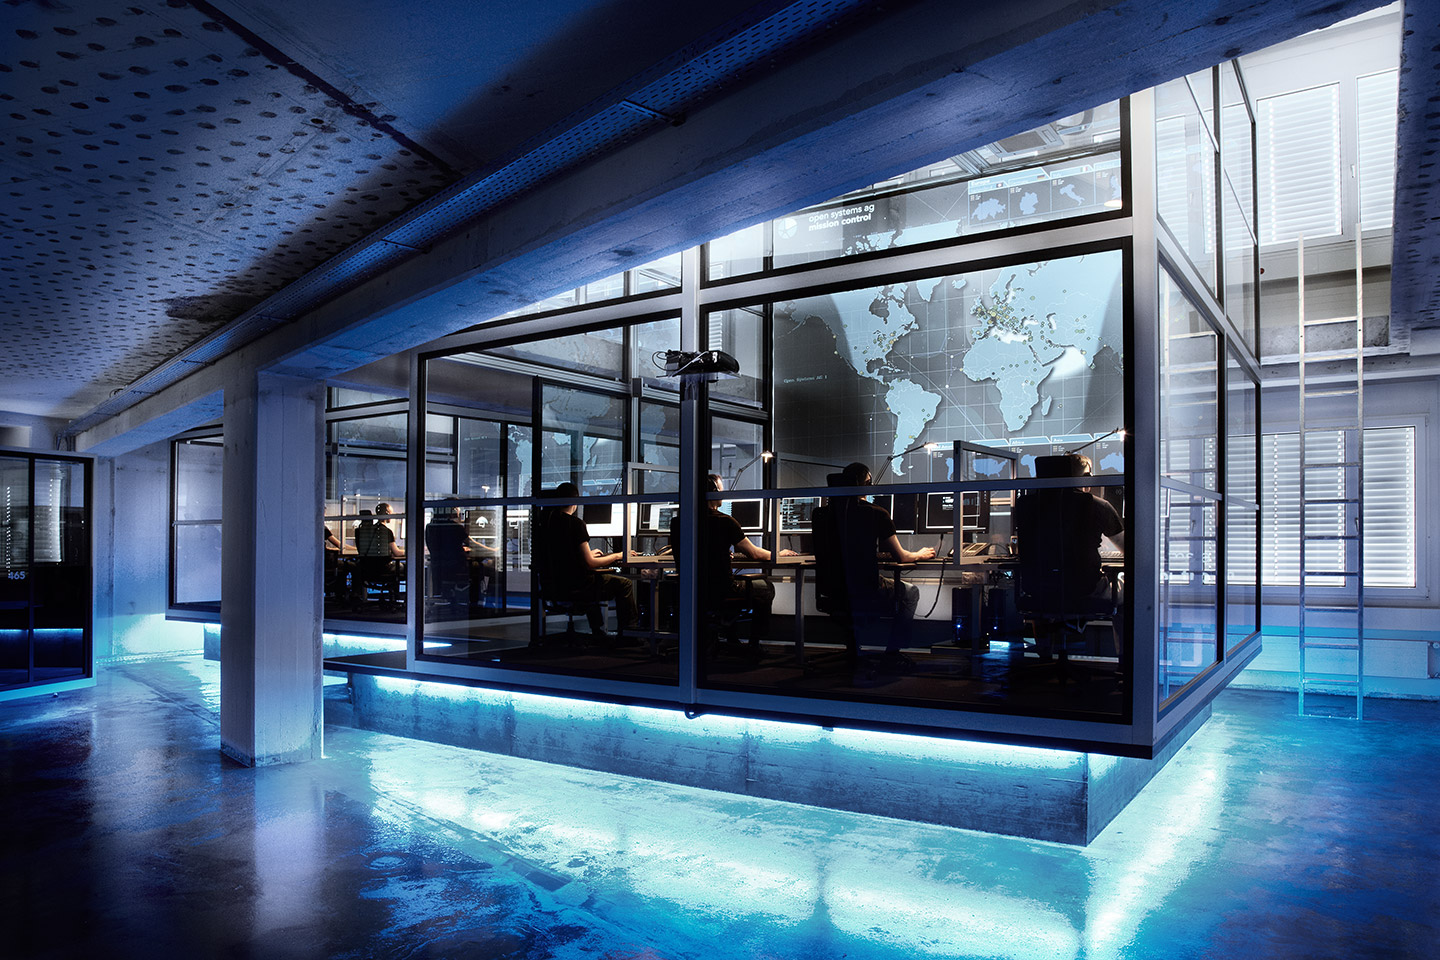
\includegraphics[clip,scale=0.15]{mainpart/anforderungen/img/gallery_mc_01}
    \caption{Mission Control Center}
  \end{center}
\end{wrapfigure}

Die Firma \osag betreibt ein weltweites Netz von \acs{IPsec} \acs{VPN} Verbindungen. Die Kunden der \osag kommen unter anderem aus den Branchen: Finanzen, Versicherungen, Regierung sowie Detail Handel. Daher ist es für \osag sehr wichtig, dass die Verbindungen konstant überwacht werden. Zu diesem Zweck wird auch ein Mission Control Center betrieben dass den Betrieb der \acs{VPN} Tunnels 24/7 überwacht. Dieses Mission Control Center\footnotemark[1] ist zuständig, dass periodische Tests der Verbindungsqualität gemacht werden sowie akute Probleme direkt erkannt und behoben werden. Das manuelle Überprüfen von Paket-Verlusten und bestimmen von Fragmentierungsproblem nimmt viel Zeit in Anspruch. Es soll nun eine Applikation programmiert werden, womit sich diese Arbeit automatisieren lässt, sodass mit weniger Aufwand eine bessere Verbindungsqualität gewährleistet werden kann.

\footnotetext[1]{Bild: \url{http://open.ch}}

\subsection{Produktfunktion}
Mit dem Tool soll das Erkennen und Diagnostizieren von Problemen bei \acs{IPsec} \acs{VPN} Verbindungen vereinfacht werden. Dabei soll das \tool{} die Möglichkeit bieten passiv Paket-Verluste zu erkennen sowie aktiv die \acs{MTU} zu bestimmen. Die Applikation ist als konstant laufender Service konzipiert und bietet daher keine graphische Oberfläche sondern nur ein Commandline-Interface. Für die Kommunikation mit den Benutzern des Tools sollen Log-Einträge verwendet werden.

\subsection{Benutzercharakteristik}
Die Benutzer des \tool{} sind Netzwerkadministratoren und Entwickler die \acs{IPsec} \acs{VPN} Tunnels betreiben. Daher kann ein gutes Mass an technischem Verständnis und Erfahrung bei der Verwendung von Commandline-Applikationen gerechnet werden.

\subsection{Abhängigkeiten}
Das \tool{} ist grundsätzlich eine eigenständige Applikation. Es wurde jedoch bereits in der Ausschreibung dieser Arbeit festgelegt dass libpcap als Library für das Capturen von Paketen verwendet werden soll. Daher ist das \tool{} von libpcap und einem entsprechenden Wrapper abhängig.
\section{Use Cases}
\label{sec:Use Cases}
todo

\subsection{Aktoren \& Stakeholder}
ddd

\subsection{Manual testing}
fff

\section{Funktionale Anforderungen}
\label{sec:Funktionale Anforderungen}

\todo{Detaillierte Beschreibung der Kriterien mit fliesstext..}

\subsection{Muss-Kriterien}
\begin{itemize}
  \item M0: Paket-Verlust messen
  \item M1: MTU bestimmen
  \item M2: Log-Nachrichten schreiben
  \item M3: Programm ist konfigurieren
\end{itemize}

\subsection{Soll-Kriterien}
\begin{itemize}
  \item S0: Unterstützung von mehreren Tunnels
  \item S1: Applikation läuft permanent als Daemon/Service
  \item S2: Konfiguration ist Machinen und Menschen lesbar
\end{itemize}

\subsection{Kann-Kriterien}
\begin{itemize}
  \item K0: Die Applikation liest die benötigte Konfiguration aus vorhandenen Konfigurationsfile für die \acs{IPSec} Tunnels aus.
  \item K1: Es können direkt aus dem \tool Statistiken gezogen werden.
\end{itemize}
\section{Nichtfunktionale Anforderungen}
\label{sec:Nichtfunktionale Anforderungen}

\subsection{Angemessenheit}
\begin{itemize}
\item Es sollen alle der genannten Muss \& Soll Kriterien erfüllt werden.
\item Alle in den Use Cases beschriebenen Anwendungsfälle sollen durch den User des \tool{}s ausgeführt werden können.
\item Die Applikation soll schlank und in einem einheitlichen Stil programmiert werden. Zudem sollen die Vorschriften der Codeformatierung von Go übernommen werden. Dadurch wird eine höhere Übersichtlichkeit und leichtere Einarbeitung in den Code gewährleistet.
\end{itemize}

\subsubsection{Funktionalität}
\begin{itemize}
\item Das Window für die Gültigkeit von \ac{ESP} Paketen ist konfigurierbar. Die Konfiguration führt zu einer individuelleren Erkennung von Paketverlusten. So kann auch bestimmt werden ab welcher Abweichung verspätetes Paket als verloren angesehen wird.
\item Das Diagnose Tool funktioniert mindestens bis zu einer Datenrate von 300Mbit/s.
\item Es ist konfigurierbar welches Netzwerkinterface bei der Überwachung verwendet werden soll.
\end{itemize}

\subsubsection{Testbarkeit}
\begin{itemize}
\item Die Businesslogik soll über alle Use Cases (Normal Verhalten) mit automatischen Unit-Tests abgedeckt sein.
\item Für die Unit Tests soll die "testing" Package von Go verwendet werden. Mithilfe dieser Package lassen sich Unit Tests schreiben die automatisch ausgeführt werden und so bei jeder Änderung Feedback zur Integrität der Applikation geben.
\end{itemize}

\subsubsection{Fehlertoleranz}
\begin{itemize}
\item Das System muss auch nach einem Neustart in einem definierten Zustand sein. Dies auch bei einem unvorhergesehenen Abbruch des Programms. 
\item Um eine Fehlerhafte Ausführung und damit verbundene Schäden zu vermeiden, wird vor dem Start überprüft ob die eingestellte Konfiguration gültig ist.
\end{itemize}

\subsubsection{Änderbarkeit}
\begin{itemize}
\item Konfiguration, Daten und Reports werden in einem Standard gespeichert, welcher auch von anderen Systemen gelesen werden kann (z.B. CSV, XML, JSON).
\item Der Code inklusive Kommentar sind auf Englisch um eine leichtere Anpassbarkeit zu erreichen.
\end{itemize}

\subsubsection{Anforderungen an Umgebung}
\begin{itemize}
\item Das Tool ist unter dem Betriebssystem Linux lauffähig, es werden jedoch Root-Rechte benötigt.
\item Für die Ausführung des \tool{}s ist eine Installation der \ac{PCAP}-Library libpcap notwendig.
\item Für das Kompilieren des \tool{}s ist eine Go-Entwicklungsumgebung notwendig.
\item Das \tool{} ist Open Source und der Quellcode wird frei verfügbar unter der MTI Lizenz veröffentlicht.
\end{itemize}
% Summary index document for the analysis chapter
\chapter{Analyse}
\label{chap:Analyse}

In diesem Kapitel wird unsere Wahl der Programmiersprache und \acs{PCAP}-Library erläutert.

\section{Einführung}
Gemäss der Aufgabenstellung dieser \work ist die Programmiersprache für das \tool frei wählbar mit der einzigen Voraussetzung dass man eine \acs{PCAP}-Library einbinden kann. In der Inception-Phase des Projekts ging es daher darum eine geeignete Sprache und Bibliothek zu wählen.

\section{JNetPcap}
\label{sec:JNetPcap}

todo Jan

\section{Golang und goPacket}
\label{sec:Golang und goPacket}

\subsection{Golang}
Golang, auch Go genannt, ist eine eher junge Programmiersprache seit 2007 von Google Inc. entwickelt wurde. Golang hat einen C-ähnlichen Syntax, bietet aber viele Eigenschaften von modernen Programmiersprachen wie zum Beispiel Garbage Collection, Type-Safety, Dynamic-Typing, Closures und eine grosse Standard-Library.
Im Oktober 2009 wurde die Golang der Öffentlichkeit als Open Source zur Verfügung gestellt.

\subsection{Evaluation}
Unseren ersten Kontakt mit Golang haben wir durch GoProbe von Open Systems gewonnen.
GoProbe erlaubt leichtgewichtiges aggregieren von Paketen und deren effiziente Speicherung. Eine Abfrage der gespeicherten Paketen ist via Querying Flows möglich.


\section{Performance Vergleich}
\label{sec:Performance Vergleich}

\subsection{Testaufbau}
2 Desktop-Rechner der HSR sind via Gigabit-Lan miteinander verbunden. Auf den Rechnern läuft Ubuntu 14.04 x64 sowie jPerf und die jeweils getestete Software.

%todo Grafik mit MS Visio die unser Testaufbau darstellt.

\subsection{Testdurchführung}
Auf einem der beiden Rechnern läuft jeweils jPerf im Server-Modus sowie die getestete Software. Auf dem anderen Computer läuft jPerf im Client-Modus.
Via. jPerf wird nun soviel Traffic erzeugt um die 1Gbit/s-Leitung möglichst stark auszulasten, d.h. durchschnittlich 900mbit/s. Die getestete Software zeichnet dabei die ganzen Pakete auf und sollte dabei 300mbit/s an Traffic ertragen können. 300mbit/s sind gem. Open Systems AG die Lastspitzen mit denen etwa zu rechnen sind.

\subsection{Ergebnisse}
Java und Golang sind von den Ergebnissen her recht ähnlich. Beide haben die Anforderung von 300mbit/s erfolgreich erfüllt. Golang ist mit den Durchschnittlich 17\% CPU Auslastung etwas performanter als Java. Die 31\% CPU Lastspitze bei Java gibt es jeweils nur wenn das Programm zum ersten Mal gestartet wird und kommt daher dass dann die ganze \acs{JVM} zuerst hochgefahren werden muss.
Beim Memory siehts bei goProbe klar besser aus weil es den ganzen \acs{JVM} Overhead nicht hat.

\begin{table}[h]
\begin{tabular}{|l|l|l|l|}
\hline
\rowcolor[HTML]{C0C0C0} 
\textbf{Software} & \textbf{CPU Spitze} & \textbf{CPU Ø} & \textbf{Memory Ø} \\ \hline
JNetPcap auf Java & 31\%                & 20\%           & tbd               \\ \hline
goProbe auf Go    & 18\%                & 17\%           & tbd               \\ \hline
\end{tabular}
\end{table}

\section{Entscheidung}
Open Systems AG würde es bevorzugen wenn wir Golang statt Java einsetzen. Die Ergebnisse des Performance-Tests sprechen ebenfalls für Golang. Und wir haben durchaus auch das Interesse einmal eine neue Programmiersprache zu lernen.
In Anbetracht dessen haben wir uns entschieden das \tool mit Golang zu entwickeln.
%todo strongswan?/Ipsec aufbau
%% Summary index document for implementation
\chapter{Implementation}
\label{chap:Implementation}

\section{Einleitung}
In diesem Kapitel wird die Architektur des \tool{} genauer erläutert und die Implementierung der beiden Hauptfunktionen: \enquote{Erkennen von Paket-Verlust} und \enquote{Bestimmen der \acs{MTU}} aufgezeigt.

\section{Aufbau der Applikation}
\label{sec:Aufbau der Applikation}

\subsection{Einleitung}
Zur Entwicklung des \tool{}s wird wegen den im Kapitel Analyse erläuterten Gründen die Programmiersprache Go eingesetzt. Go erlaubt zwar einen Objekt-Orientierten Stil des Programmieren \cite[:240]{golang_faq}, bietet aber im Vergleich zu typisch \acs{OOP} Sprachen wie Java oder C++ keine Klassen \& Typen Hierarchie.

Anstatt von Klasse als Struktur bietet Go sogenannte Packages an. Innerhalb einer Package können beliebig viele \code{.go} Files erstellt werden, die dann den Source Code enthalten. Private Variablen und Funktionen sind innerhalb einer Package frei zugänglich, können aber ausserhalb der Package nicht aufgerufen werden.

\begin{lstlisting}[language=bash, caption=Package Struktur des \tool{}]                    
github.com/ipsecdigatool/ipsecdigatool/       
	.git/
	capture/ # Pakete von Netzwerkadapter capturen        
		capture.go
	config/ # Konfiguration erstellen, laden, aktualisieren
		config.go
	logging/ # Syslog Nachrichten absetzen
		logging.go
	mtu/ # MTU Discovery durchfuehren
		analyze.go
		capture.go
		send.go
	packetloss/ # Packet loss feststellen
		detect.go
		espmap.go
		lostfile.go
	main.go # Programmstart und Daemon Funktionalitaet
\end{lstlisting}

Die Packages \code{capture}, \code{config}, \code{logging} werden sowohl für die \acs{MTU} Discovery als auch für die Packet Loss Detection verwendet. Die Packages \code{mtu} und \code{packetloss} werden nur für die jeweiligen Funktionen gebraucht und sind unabhängig voneinander. Das \code{main.go} enthält allen Code der für den Programmstart sowie den Daemon Mode gebraucht wird.

\subsection{Namenskonvention}
Go unterscheidet öffentliche und private Funktionen und Variablen durch die Grosse- oder Kleinschreibung des ersten Buchstaben eines Funktions- oder Variablennamens. Gross geschriebene Namen zeigen eine öffentliche Funktion oder Variable an, die dann auch ausserhalb der Package genutzt werden kann.
In der Go Usergroup ist ausserdem auch die Idee verbreitet, dass Variablen- und Funktionsnamen möglichst kurz und prägnant sein sollen. CamelCase Namen sollen nach Möglichkeit vermieden werden. Dies kommt wohl einerseits von der C-Ähnlichkeit hat aber andererseits auch einen praktischen Grund. So ist ein Funktionsaufruf wie \code{capture.Start()} tatsächlich recht elegant und gut verständlich.
Im Verlauf dieses Projekts haben wir auch festgestellt, dass es besser ist alle Namen, Ordnernamen und Kommandos wenn möglich klein zu schreiben. Zu Beginn des Projekts haben wir \code{github.com/IPsecDiagTool/IPsecDiagTool} als Repository Ordner Struktur verwendet und dies hat zu einigen Konflikten geführt. Glücklicherweise lassen sich Repositories auf github.com relativ leicht umbenennen und wir konnten auf eine rein klein geschriebene Ordner Struktur umsteigen.

\subsection{Programmstart \& Multi-Threading}
Am Programmstart des \tool{} lässt sich das Zusammenspiel der verschiedenen Packages beobachten. Zuerst wird jeweils die Konfiguration geladen. Falls kein Konfigurationsfile auf dem System vorhanden ist wird ein neues File mit Default Werten erstellt. Danach werden die \code{logging} und \code{mtu} Packages initialisiert.

\begin{figure}[ht]
    \begin{center}
    % GFX Trim left bottom right top
        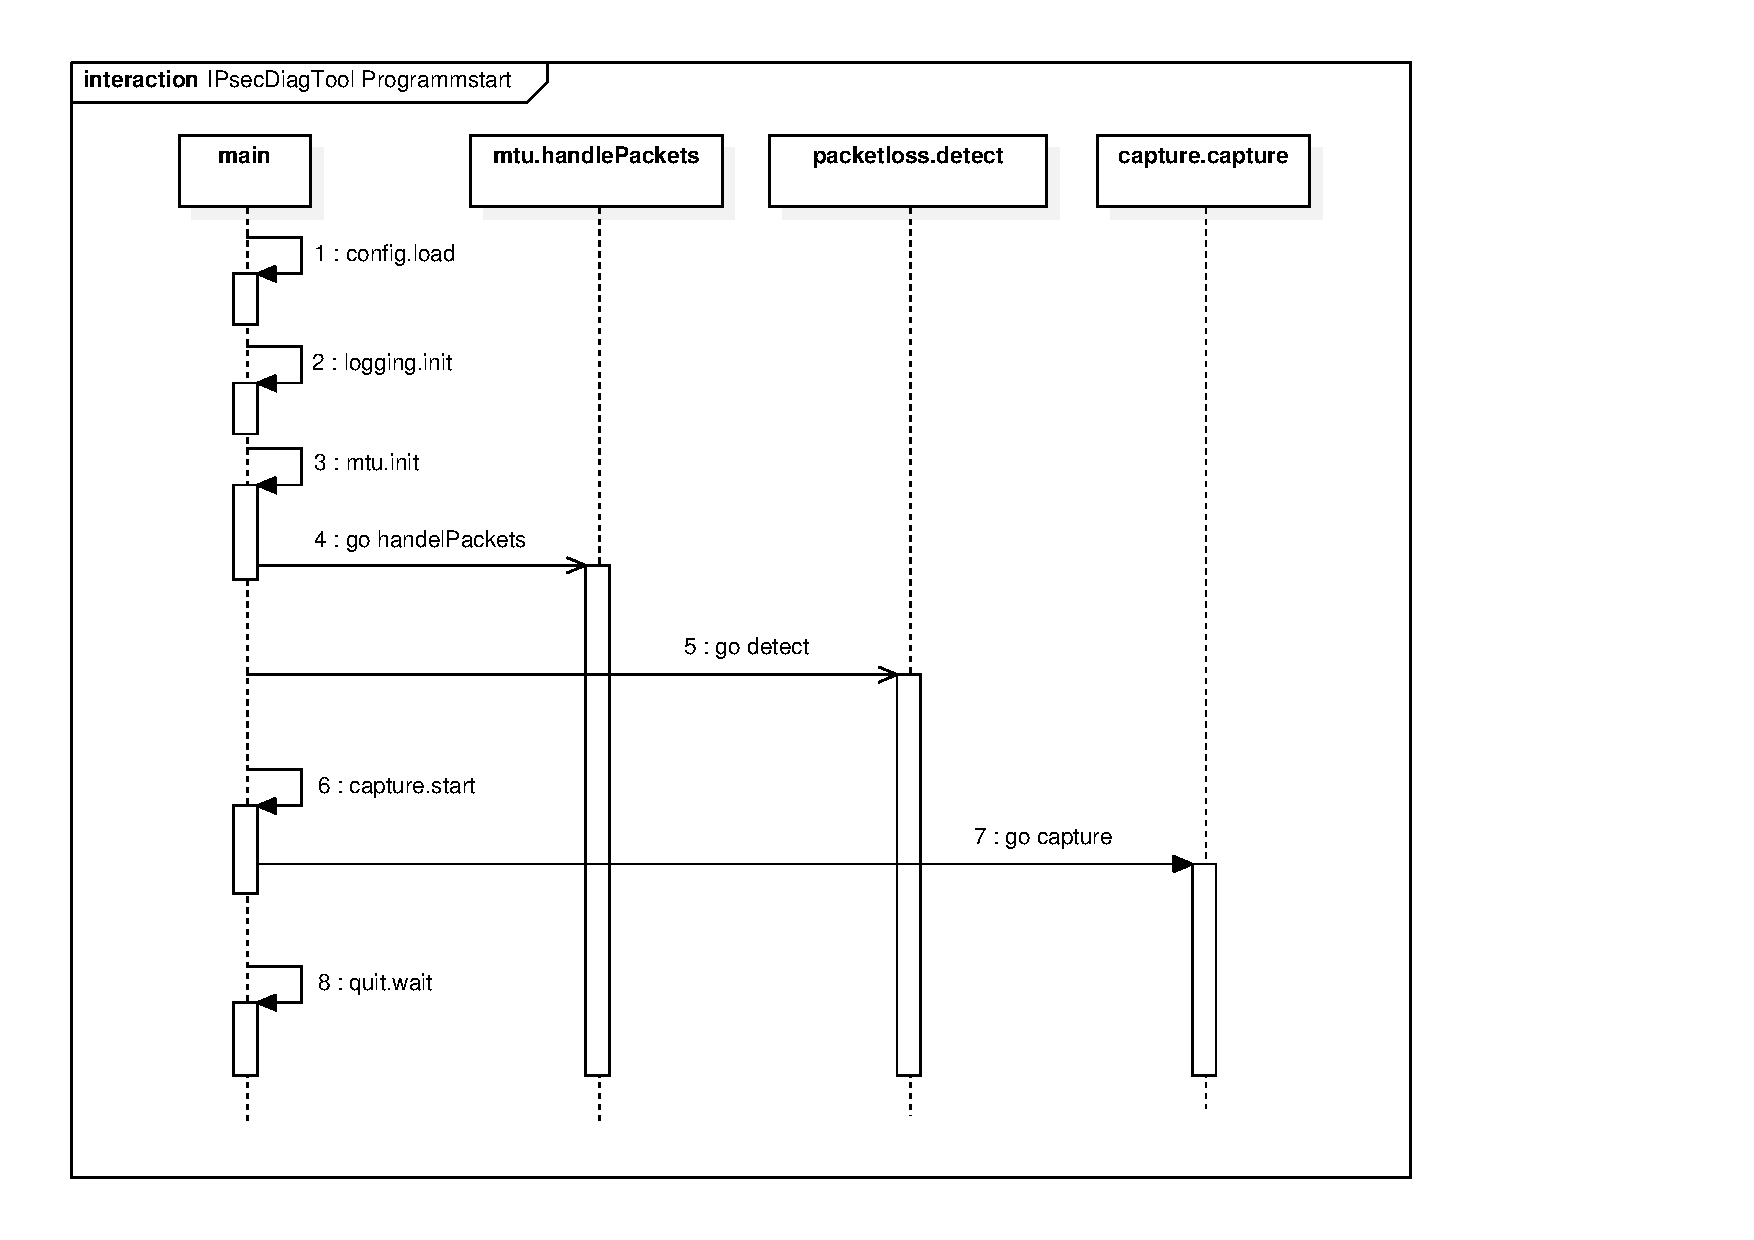
\includegraphics[trim=30 20 150 30,clip,width=\textwidth]{mainpart/implementation/img/programmstart}
    \end{center}
    \caption{Programmstart des \tool{}}
\end{figure}

Beim Initialiserungs-Vorgang der jeweiligen Package werden die fürs Multi-Threading notwendigen Konstrukte erstellt. Bei Go wird Multi-Threading vor allem via Goroutinen und Channels realisiert. Eine Goroutine ist eine Funktion die im gleichen Address Space, gleichzeitig mit anderen Goroutinen ausgeführt wird. Goroutinen sind leichtgewichtig und kosten bei der Erstellung nicht mehr als Stack Space. Um Nebenläufigkeit zu erreichen, werden Goroutinen auf mehrere Threads des Betriebsystems multiplexed. Wenn eine Goroutine blockiert, können die anderen Goroutinen weiterlaufen \cite[:1391]{effective_go}.
Zur Synchronisation und zum Datenaustausch zwischen Goroutinen werden sogenannte Channels verwendet. Typischerweise hat man in einer Goroutine eine for-Schleife und wartet darin auf Input aus einem Channel.

Nachdem Initialisieren werden die Goroutinen der \code{mtu} und \code{packetloss} Packages gestartet. Zum Schluss wird die \code{capture} Goroutine gestartet. Ab jetzt werden die Pakete vom konfigurierten Interface aufgezeichnet und vom \tool{} verarbeitet. Die Main Funktion ist nur noch dafür verantwortlich ein vom User gesendetes \code{SIGTERM} Signal abzufangen und gegebenenfalls das Programm zu beenden.

\subsection{Pakete einfangen}
Das Einfangen von Paketen mit \ac{PCAP} ist in der \code{capture} Package implementiert. Sie bietet nur eine öffentliche Funktion die via \code{capture.Start(..)} aufgerufen werden kann. Als Parameter nimmt die Funktion die Konfiguration sowie ein Channel für \ac{ICMP}s und ein Channel für \ac{ESP}s entgegen. 

Wenn die Funktion \code{capture.Start(..)} aufgerufen wird, werden die benötigten Variablen in der \code{capture} Package initialisiert und danach eine separate Goroutine mit der \code{capture.capture(..)} Funktion gestartet. Die \code{capture.Start(..)} Funktion ist blockierend bis die \code{capture.capture(..)} Goroutine gemeldet hat, dass sie bereit ist. \code{Capture.Start(..)} gibt ein Channel zurück, der verwendet werden kann, um die \linebreak \code{capture.capture(..)} Goroutine zu beenden.

\begin{lstlisting}[language=go, caption=Öffentliche Funktion capture.Start()]     
func Start(c config.Config, icmpPackets chan gopacket.Packet, ipsecESP chan gopacket.Packet) chan bool {
	initChannels(icmpPackets, ipsecESP)
	quit := make(chan bool)
	captureReady := make(chan bool)
	go capture(c.PcapSnapLen, quit, captureReady, c.PcapFile)
	<-captureReady
	if c.Debug { log.Println("Capture Ready.") }
	return quit
}
\end{lstlisting}

In der \code{capture.capture(..)} Funktion findet das eigentliche Einfangen von Paketen statt. Zuerst wird ein \code{pcap.Handle} erstellt. Dafür hat man beim gopacket Wrapper zwei Möglichkeiten. Zum einen kann man mit \code{pcap.OpenOffline(file)} ein Handle auf eine \ac{PCAP}-Datei erstellen. Oder aber man erstellt einen Handle auf ein Netzwerk-Interface mit \code{pcap.OpenLive(\enquote{any}, snaplen, true, 250*time.Millisecond)}. In diesem Beispiel wurde das Interface \enquote{any} verwendet. Das heisst Pakete von allen Netzwerk Interfaces werden eingefangen. Die \code{snaplen} Variable deklariert wie lange ein eingefangenes Paket maximal sein darf. Wenn das Paket die \code{snaplen} überschreitet, wird es abgeschnitten. Dann muss noch angegeben werden ob dass Interface im \enquote{promiscuous mode} laufen soll und zu guter Letzt noch ein Timeout Wert. Ist ein Timeout Wert gesetzt wird jeweils so lange gewartet bevor die eingefangenen Pakete weitergegeben werden. Dies hilft die Performance zu verbessern.

Wenn der Handle erstellt wurde, wird daraus eine PaketSource gemacht. Diese PaketSource kann nun in einer for-Schleife verwendet werden und liefert fortwährend die eingefangenen Pakete. In dieser for-Schleife wird dann entschieden, ob ein eingefangenes Paket ein \ac{ESP} oder aber ein \ac{ICMP} ist. Falls eines der beiden zutrifft, wird es in den entsprechenden Channel gelegt. Wenn das Paket weder \ac{ESP} noch \ac{ICMP} ist, wird es verworfen. Die for-Schleife läuft so lange, bis eine Nachricht in den quit-Channel gelegt wird.

\begin{lstlisting}[language=go, caption=Einfangen und Verteilen von Paketen]    
packetSource := gopacket.NewPacketSource(handle, handle.LinkType())
captureReady <- true

for {
	select {
	case packet := <-packetSource.Packets():
		if packet != nil {
			if packet.Layer(layers.LayerTypeIPsecESP) != nil {
				putChannel(packet, ipsecChannel)
			}
			if packet.Layer(layers.LayerTypeICMPv4) != nil {
				putChannel(packet, icmpChannel)
			}
		}
	case <-quit:
		log.Println("Received qu..") return nil
	}
}
\end{lstlisting}
\clearpage

\section{Paketverlust erkennen}
\label{sec:Paketverlust erkennen}

\subsection{ESP Aufbau}
\noindent Encapsulating Security Payload (ESP) wird bei IPsec (VPN) eingesetzt. Es gewährleistet die Vertraulichkeit und Integrität von Paketen und kümmert sich um die Authentisierung. Durch diese Integritätssicherung werden Pakete vor Manipulation geschützt.ESP verschlüsselt, im Unterschied zu Authentication Header (AH), die Nutzdaten. Bei AH werden nur die Integrität und Echtheit sichergestellt.

\noindent http://www.elektronik-kompendium.de/sites/net/1410261.htm

\noindent Der ESP header wird zwischen dem IP header und dem darunterliegenden Protokoll eingefügt (transport mode), oder es kapselt das ganze IP-Paket (tunnel mode).

\noindent RFC 2406

\noindent Der tunnel mode wird vor allem bei der Verbindung zwischen zwei Netzwerken über eine unsichere Verbindung eingesetzt. Der Modus unterstützt aber prinzipiell alle Arten von VPN-Anwendungen.Bei dieser Verwendung wird das ganze IP-Paket verschlüsselt und in ein neues IP-Paket verpackt. So wird das gesamte Paket durch ESP abgeschirmt und die eigentliche IP-Adresse des Absenders ist nicht mehr ersichtlich.Diese Methode hat natürlich einen gewissen Overhead. Es kommen 8 Byte für den ESP-Header, 16-20 Byte ESP-Trailer und für den neuen IP-Header 20 Byte hinzu.


\noindent Grafik für Tunnelmode
\noindent http://www.elektronik-kompendium.de/sites/net/1410261.htm

\noindent Bei einer Situation in der nur zwei Rechner miteinander verbunden werden, kann der Transportmodus verwendet werden. Dieser Modus unterstützt nur Host-to-Host Verbindungen. Da es für IPsec nicht unbedingt notwendig ist IP-Pakete vollständig neu zu enkapeln, können beim transport mode der originale IP-Header verwendet werden.Es kommen 8 Byte ESP-Header und 16-20Byte ESP-Trailer hinzu. Damit wird der Overhead kleiner, da man keinen zusätzlichen IP-Header benötigt.

\noindent Grafik für Transportmode

\noindent http://www.elektronik-kompendium.de/sites/net/1410261.htm

\noindent Wichtige Felder

\noindent Security Parameters Index (SPI) 32bits

\noindent Dieser willkürlich festgelegte Wert in Kombination mit der IP-Adresse des Ziels wird für eine Identifikation der Verbindung benötigt. Bei jeder neuen Verbindung wird die SPI neu gesetzt.

\noindent Sequence number 32bits

\noindent Die Sequence number wird für jedes Paket gesetzt und wird danach für jedes neue Paket um 1 erhöht. Bei einer neuen Verbindung wird die Sequece number stets auf 1 gesetzt.Falls Anti-Replay eingesetzt wird (standardmässig aktiviert) darf sich die Sequence number nicht wiederholen. Daher wird bevor das 2\^{}32 paket gesendet wird die Verbindung zurückgesetzt und eine neue SPI ausgehandelt. Damit wird auch die Sequence number wieder zurückgesetzt.

\noindent 


\subsection{Vorgehen bei Paketverlust}

{\raggedright
Falls ein \"{U}bertragungsmedium nicht korrekt funktioniert ist es m\"{o}glich,
dass Datenpakete nicht am Ziel ankommen oder mit einer zu grossen Versp\"{a}tung.
Da jedes \esp Paket mit einer Sequenznummer versehen ist, k\"{o}nnen diese
Paketverluste erkannt und gemeldet werden.
}

{\raggedright
Die \esp Pakete Besitzen zum Schutz vor Replay-Angriffen eine Sequenznummer sowie
einen bestimmten G\"{u}ltigkeitsbereich (Windowsize).
\\
Die Pakete k\"{o}nnen zum Beispiel durch Loadbalancing \"{u}ber unterschiedliche
Pfade verschickt werden. Dadurch kann die Reihenfolge der Pakete am Ziel nicht
mehr gew\"{a}hrleistet werden. Die zu sp\"{a}t ankommenden Pakete m\"{u}ssen
daher \"{u}berpr\"{u}ft werden, ob die Sequenznummer aktuell noch g\"{u}ltig ist
(innerhalb des Window).
}

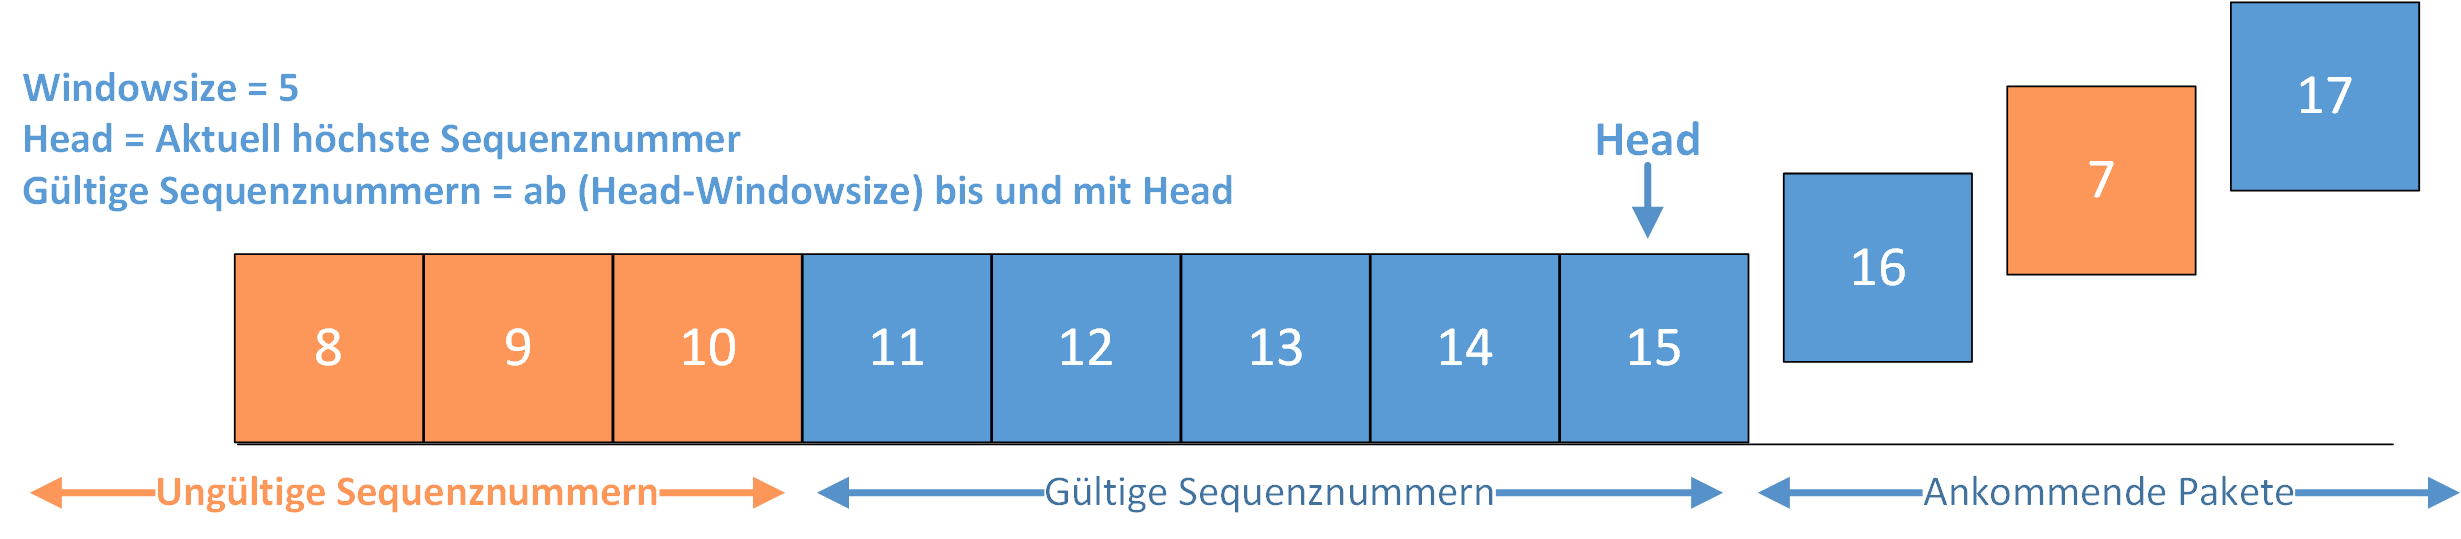
\includegraphics[width=1\textwidth]{start/img/Sequenznummern.png}

\subsection{Datenstruktur für die \esp Verbindungen}
Da pro Verbindung separate Sequenznummern verwendet werden, werden die verschiedenen Verbindungen durch eine Hashmap verwaltet. Als Key wird eine Struktur aus Source, Destination und \acs{SPI} verwendet. Als Value werden grundsätzlich zwei Listen für die Lost und MaybeLost Pakete benötigt. Zusätzlich wird noch ein Wert für den aktuellen Head gespeichert.

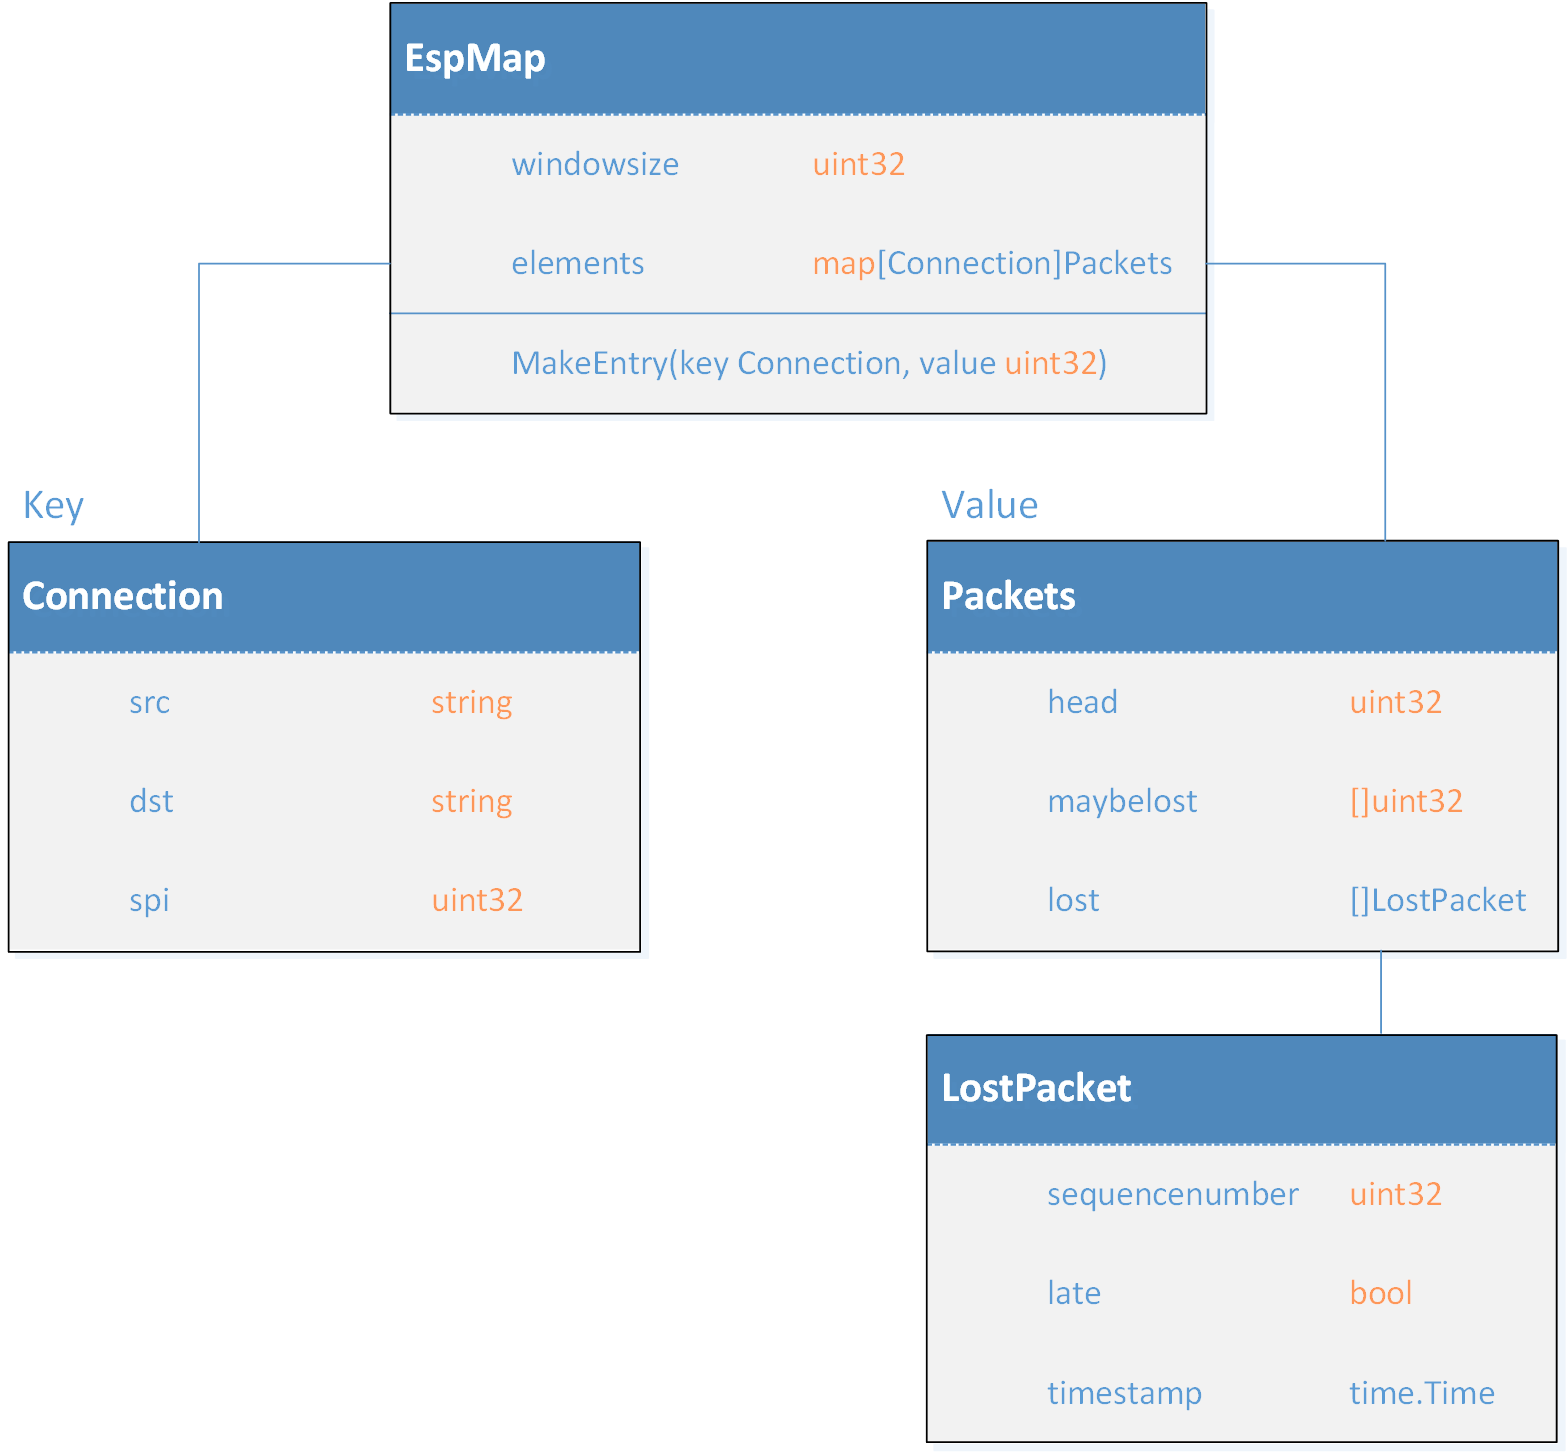
\includegraphics[width=1\textwidth]{start/img/Datenstruktur.png}

\subsection{Erkennung des Paketverlusts}
Die Paketverluste werden mit folgendem Algorithmus festgestellt.
Vereinfachte Darstellung des Algorithmus in Pseudocode:
\\
\textbf{Neues Packet Verarbeiten}
\begin{lstlisting}[language=go]
if(neuesPacket > Head){
	if(neuesPacket != Head + 1){
		Packete von Head bis neuesPacket in 
		MaybeLost speichern
	}
	Head = neuesPacket
	CheckLost()
}else{
	if(Head-WindowSize < neuesPacket){
		Packet aus MaybeLost entfernen
	}else{
		Flag fuer zu spaet angekommen setzen	
	}
}
\end{lstlisting}

\textbf{CheckLost}
\begin{lstlisting}[language=go]
for(MaybeLost){
	if(Head-WindowSize >= MaybeLostEintrag){
		Packet in Lost Speichern
		Packet aus MaybeLost entfernen
	}
}
\end{lstlisting}


\section{Syslogprotokoll}
\label{sec:Syslogprotokoll}

\noindent Syslog ist eines der am häufigsten eingesetzten Protokolle zum Übermitteln von Log-Meldungen in einem Netzwerk. Durch den einfachen Aufbau und die breite Unterstützung ist es leicht einsetzbar.


\subsection{ Aufbau}

\noindent Eine Syslog-Meldung besitzt ein Severity-Field womit der Schweregrad einer Nachricht festgelegt werden kann.

\noindent Die Werte besitzen folgende Bedeutungen:

\begin{tabular}{|p{0.5in}|p{3.7in}|} \hline 
Code & \textbf{Severity} \\ \hline 
0 & \textbf{Emergency:} system is unusable \\ \hline 
1 & \textbf{Alert:} action must be taken immediately \\ \hline 
2 & \textbf{Critical:} critical conditions \\ \hline 
3 & \textbf{Error:} error conditions \\ \hline 
4 & \textbf{Warning:} warning conditions \\ \hline 
5 & \textbf{Notice:} normal but significant condition \\ \hline 
6 & \textbf{Informational:} informational messages \\ \hline 
7 & \textbf{Debug:} debug-level messages \\ \hline 
\end{tabular}

RFC 5424

\noindent Zudem besteht eine Meldung noch aus einem Header sowie der eigentlichen Nachricht.

\noindent 


\section{ Meldungsaufbau}

\noindent Die Bedingungen für das Auslösen eines Alerts können im Configfile festgelegt werden. Es können der Zeitraum und die Anzahl Pakete definiert werden. Falls innerhalb dieses definierten Zeitraums die Anzahl an verlorenen Paketen überschritten wird, wird ein Alert ausgelöst.

\noindent Der Alert besitzt folgende Form:

\begin{tabular}{|p{0.5in}|p{0.7in}|p{3.0in}|} \hline 
Severity & Programm & Meldung \\ \hline 
1 & IpsecDiagTool & Too much LostPackets in Connection: (SPI: \dots ,SRC:\dots ,DST\dots ) \\ \hline 
\end{tabular}



\noindent So kann gleich anhand der Meldung erkannt werden um welche Verbindung es sich handelt und die notwendigen Schritte für eine Korrektur vorgenommen werden.

\noindent Damit es nicht zu einer Flut von Benachrichtigungen mit dem gleichen Inhalt und den gleichen Paketen kommt, wurde ein Timer von 10 Sekunden eingeführt.


\section{ Logging Package}

\noindent Das Logging wurde in einem separaten Package umgesetzt und stellt Methoden für das Logging zur verfügung. Das Package kapselt die benötigte Funktionalität die von „log/syslog`` benötigt wird.

\noindent Das Package wird vor Verwendung der Logging Funktionalität durch InitLogger initialisiert. Dabei werden die Werte für Zeitfenster, Anzahl Packete und Syslogserver gesetzt. Danach können die Benachrichtigungen mit AlertLog und InfoLog erstellt werden.

\noindent 


\section{ Benachrichtigung mit Datei}

\noindent Gleichzeitig mit dem Syslogeintrag wird eine CSV Datei erstellt. Die Datei Beinhaltet detaillierte Informationen um welche verlorenen Pakete es sich handelt und mit welchem Abstand ein Verlust detektiert wurde. Ausserdem gibt es Informationen ob ein Paket möglicherweise zu spät eingetroffen ist (also ausserhalb des Windows für die Sequenznummern). Falls dieses Problem vermehrt eintritt könnte ein erhöhen der Windowsize nötig sein.

\noindent Die Datei wurde so angepasst, dass sie mit Microsoft Excel oder ähnlichen Programmen problemlos gelesen und weiter verarbeitet werden kann.

\noindent 

\noindent Beispiel einer Datei

\begin{tabular}{|p{0.9in}|p{1.7in}|p{0.8in}|} \hline 
\multicolumn{2}{|p{1in}|}{SPI:12345 SRC: 192.168.0.1 DST: 192.168.0.2} &  \\ \hline 
Sequencenumber & Timestamp & ReceivedLater \\ \hline 
2 & Monday, 04-May-15 11:53:42 CEST & false \\ \hline 
3 & Monday, 04-May-15 11:53:42 CEST & true \\ \hline 
4 & Monday, 04-May-15 11:53:42 CEST & false \\ \hline 
5 & Monday, 04-May-15 11:53:42 CEST & false \\ \hline 
\end{tabular}



\noindent 

\clearpage

\section{MTU Discovery}
\label{sec:MTU Discovery}

\subsection{Einleitung}
Mithilfe der \acs{MTU} (Maximum Transmission Unit) wird festgelegt wie gross ein Netzwerkpaket maximal sein darf bevor es in mehrere Pakete aufgeteilt werden muss. Wenn die \acs{MTU} korrekt bestimmt wurde dann kann IP-Paket-Fragmentierung verhindert werden und die Performance der Netzwerkverbindung ist deutlich besser. In einem Netzwerk wird die \acs{MTU} typischerweise pro Netzwerk-Adapter festgelegt. Bei  \acs{IPSec} \acs{VPN} Tunnels kann die \acs{MTU} hingegen pro Tunnel definiert werden auch wenn mehrere Tunnels über den selben Netzwerk-Adapter laufen.
Typischerweise wird die MTU via \acs{PMTUD} (Path MTU Discovery) ermittelt, dabei werden \acs{ICMP} Pakete unterschiedlicher Grösse über die Verbindung gesandt und so kann festgestellt werden welches die maximale Grösse ist die noch ankommt.
Bei \acs{PMTUD} gibt es jedoch ein bedeutendes Problem. Viele Netzwerk-Sicherheits Geräte blockieren ICMP Pakete und so kann die \acs{MTU} der Verbindung nicht korrekt ermittelt werden.
Um die Probleme von \acs{PMTUD} zu umgehen und eine korrekte \acs{MTU} ermitteln zu können haben wir die MTU-Komponente des \tool entwickelt, deren Funktionsweise in den nachfolgenden Abschnitten erläutert wird.

%http://en.wikipedia.org/wiki/Path_MTU_Discovery
\todo{Citation needed}

\subsection{Path MTU Discovery}
Die Path MTU Discovery \acs{PMTUD} ist eine standardisierte Technik um die \acs{MTU} festzustellen.  Bei \acs{IPv4} funktioniert \acs{PMTUD} folgendermassen: Es werden \acs{ICMP} Pakete unterschiedlicher Grösse über die Netzwerkverbindung gesendet. Geräte deren \acs{MTU} kleiner als die Grösse des versendeten Pakets ist verwerfen das Paket und senden stattdessen eine \acs{ICMP} Nachricht mit dem Inhalt "Fragmentation Needed" zurück. So weiss der \acs{PMTUD} Algorithmus dass die versendeten Pakete noch zu gross sind um ihr Ziel zu erreichen. Die versendeten Pakete werden also verkleinert, und der Prozess wiederholt, bis eine Übertragungsgrösse gefunden wird mit der ein Paket den ganzen Pfad ohne Fragmentierung traversieren kann.

Doch wie bereits in der Einleitung angesprochen gibt es bei \acs{PMTUD} ein Problem. Viele Netzwerk-Sicherheit Geräte blockieren \acs{ICMP} Nachrichten. Dies beinhaltet die Errors "Fragmentation Needed" des \acs{PMTUD} Algorithmus. Bei der \osag wurde eben dieses Problem auch beobachtet, so gibt es \acs{VPN} Tunnels die über schlecht konfigurierte Router von Dritten laufen und so mit

%http://en.wikipedia.org/wiki/Path_MTU_Discovery
\todo{Citation needed}

\subsection{MTU-Bestimmung - Idee}
Um das Problem der blockierten \acs{ICMP} Packeten zu vermeiden bestimmt das \tool die \acs{MTU} innerhalb des \acs{VPN} Tunnels. Gegenüber den Routern die normalerweise die \acs{ICMP} Pakete blockieren würden sehen die Pakete des \tool wie normale \acs{IPSec} \acs{ESP}s aus. Sie haben jedoch wie auch die \acs{ICMP} Pakete von \acs{PMTUD} den "Don't Fragment" Flag gesetzt. Dadurch wird verhindert das die Pakete automatisch fragmentiert werden wenn sie die \acs{MTU} eines Geräts überschreiten. Im Gegensatz zu \acs{PMTUD} kann man hier nicht auf ein \acs{ICMP} "Fragmentation Needed" Paket zählen das von einer Netzwerkkomponente beim überschreiten der \acs{MTU} versendet wird. Pakete die, die \acs{MTU} überschreiben werden einfach verworfen. Deshalb muss das \tool auf beiden Seiten des \acs{VPN} Tunnels laufen und Pakete die ankommen beantworten.

Innerhalb des Tunnels wird wie bei \acs{PMTUD} auf \acs{ICMP} Pakete gesetzt. Die vom \tool versendeten Pakete enthalten eine Payload die aus den folgenden Angaben besteht:

\begin{itemize}
  \item \textbf{AppID:} Eindeutige ID des aktiven \tool. Wird verwendet um mehrere gleichzeitig laufende \tool auf einem Rechner zu unterscheiden.
  \item \textbf{ChannelID:} ID des GO-Channels von dem das Paket versendet wurde. Wird benötigt um für mehrere Tunnels gleichzeitig die \acs{MTU} festzustellen zu können.
  \item \textbf{Command:} Die eigentliche Nachricht des Pakets. z.B. "MTU?" als Request oder "OK" als Antwort.
  \item \textbf{Null-Array:} Ein mit Nullen gefülltes Array von variabler Grösse. Wird verwendet um dem Paket seine vorbestimmte Grösse zu geben.
\end{itemize}

% GFX Trim left bottom right top
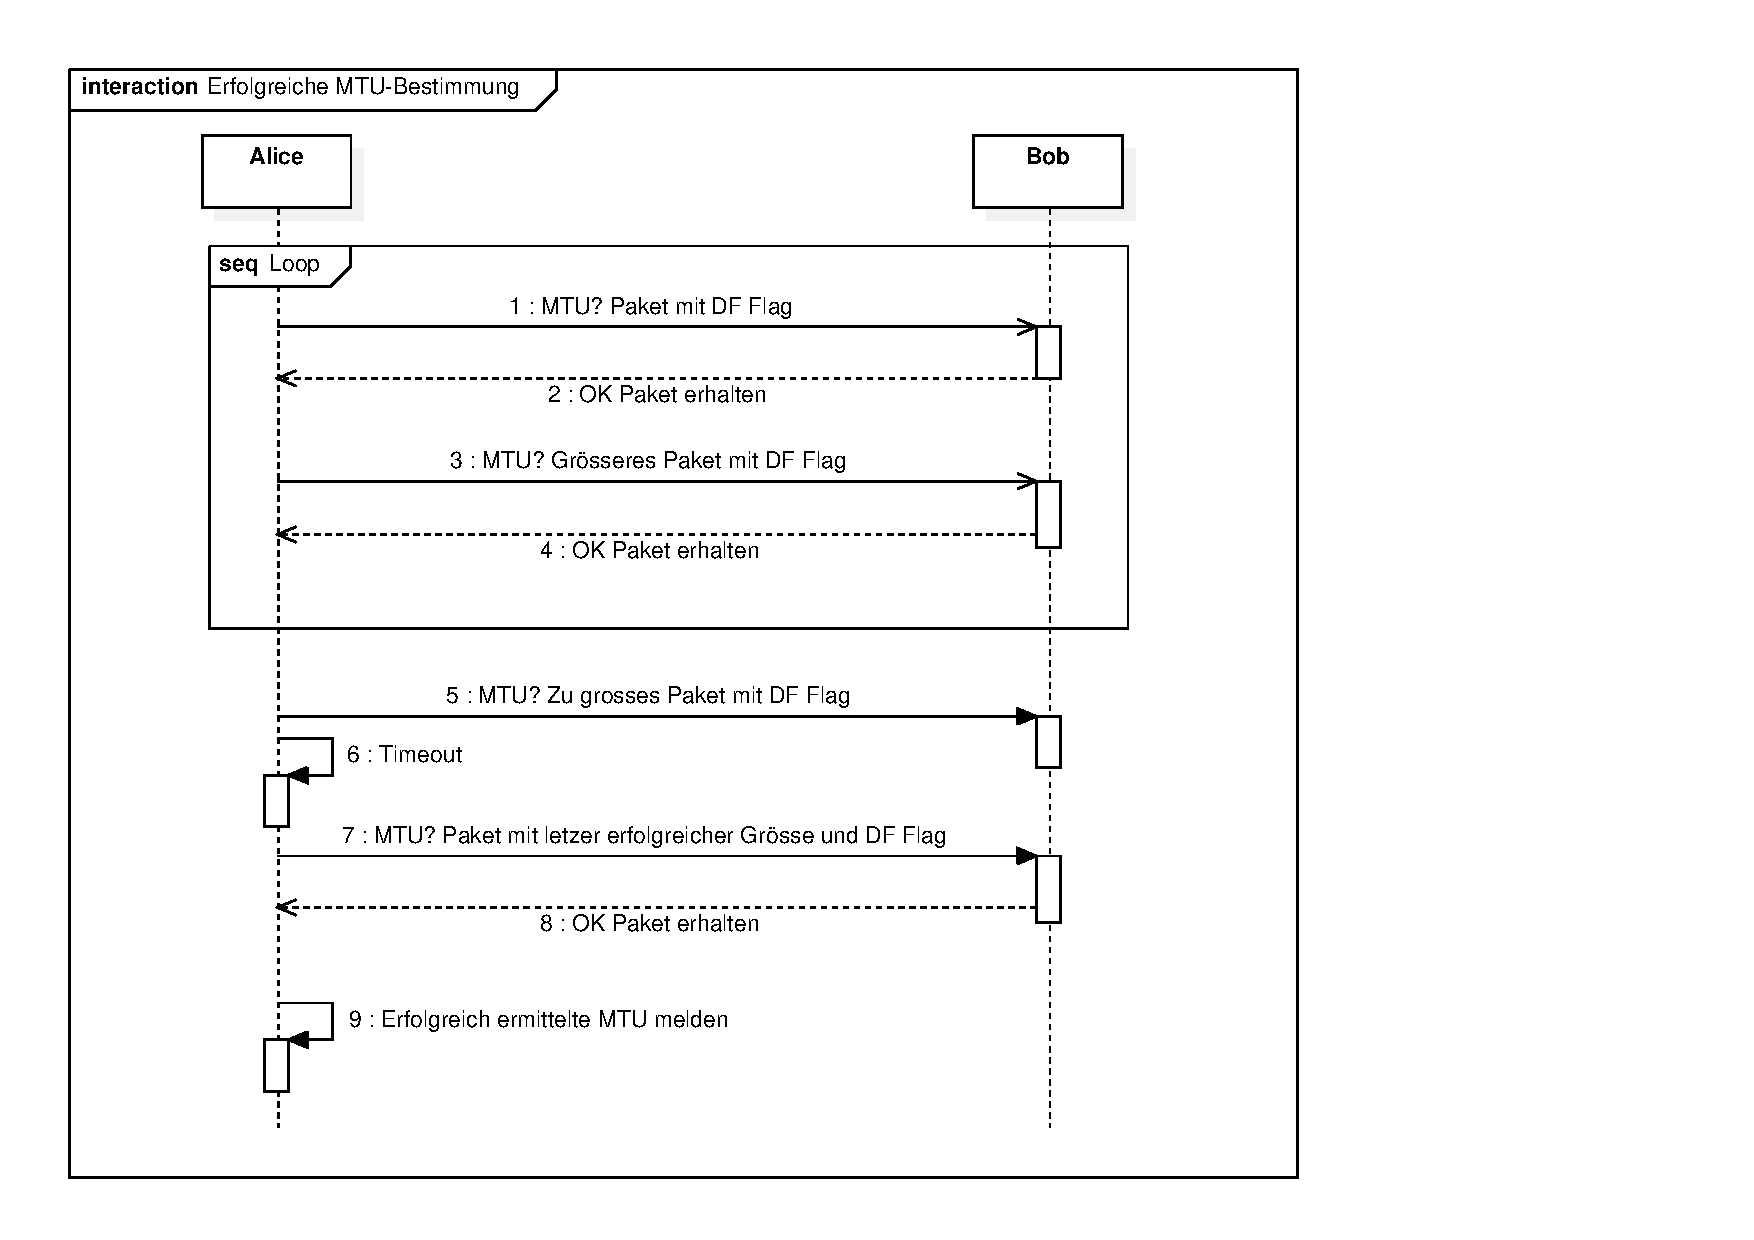
\includegraphics[trim=10 10 200 10,clip,width=\textwidth]{mainpart/implementation/img/MTUBestimmungErfolgreich}

Die obenstehende Grafik zeigt den weiteren Ablauf der \acs{MTU} Bestimmung mit dem \tool. Alice sendet ein Paket mit dem Command "MTU?" und einer bestimmten Grösse an Bob. Wenn Bob das Paket erhält, sendet er "OK als Antwort. Alice erhöht darauf die Paketgrösse und fragt Bob erneut mit "MTU?" an. Dies wird so lange wiederholt bis das Paket nicht mehr ankommt. Bob erhält also das "MTU?" Paket nicht und kann somit Alice auch keine Antwort schicken. Alice hat jedoch ein Timeout Timer und nach einer vordefinierten Zeit ohne Antwort geht Alice davon aus dass das Paket nicht angekommen ist. Alice sendet nun ein Paket mit der letzten erfolgreichen Grösse um sicher zu Stellen das die Netzwerkverbindung selbst noch besteht und protokolliert dann die letzte erfolgreiche \acs{MTU}.

\subsection{MTU-Bestimmung - FastMTU}
Die im oberen Abschnitt beschrieben Art der \acs{MTU} Bestimmung war gut als ein erster Schritt im iterativen Softwareentwicklungsprozess. Für einen produktiven Betrieb wäre sie aber nicht zu gebrauchen. Zum einen ist die oben beschriebene Variante nur exakt wenn man einen Vergösserungs-Schritt von einem Byte nimmt und wodurch der Algorithmus aber sehr langsam wird. Und zum anderen ist sie auch Anfällig auf Paket-Verluste.
Daher wurde der Algorithmus nach der ersten Iteration erweitert und überarbeitet. Die neue Variante wird von uns liebevoll "FastMTU" genannt.

Bei der FastMTU Bestimmung bleibt das grundlegende Prinzip gleich, es werden Pakete unterschiedlicher Grösse versendet so dass man herausfinden kann welche ankommen und welche verworfen werden. Neu wird jedoch nicht nur ein Paket aufs Mal versendet sondert einen ganze Batch von Paketen. Dazu wird aus der Konfiguration einen sogenannten Range ausgelesen. Der Range besteht aus zwei Byte-Grössen die festlegen worin sich die \acs{MTU} typischerweise befinden sollte. Zum Beispiel zwischen 0 und 2000 Bytes. Dann wird aus der Konfiguration ausgelesen wie viele Pakete aufs Mal versendet werden sollen. Mehr gleichzeitige Pakete führen zu einer schnelleren Bestimmung der \acs{MTU}, haben aber auch zur folge dass die Verbindung stärker belastet wird und so möglicherweise wichtiger Kunden-Traffic ausgebremst wird. Als Default-Wert gehen wir von 20 gleichzeitigen Paketen aus. Der Range 0-2000 Bytes wird jetzt also durch 20 geteilt. Damit erhält man 20 Pakete die sich je um 100 Bytes unterscheiden. Diese 20 Pakete werden nun als einen Batch versendet.
Für alle Pakete die auf der anderen Seite des Tunnels ankommen wird nun eine Antwort generiert. Bei einer MTU von 1500 Bytes würden die ersten 15 Pakete ankommen. Der Sender weiss jetzt also dass die exakte \acs{MTU} zwischen dem letzten erfolgreichen Paket (1500) und dem ersten nicht erfolgreichen Paket (1600) sein muss. 1500-1600 Bytes wird nun als nun als neuer Range gesetzt und erneut durch die Anzahl gleichzeitiger Pakete geteilt. Die Pakete des zweiten Batches haben also noch 5 Byte Unterschied. Dieser Vorgang wird so lange wiederholt bis der Unterschied zwischen den Paketen eines Batches nur noch 1 Byte sind. Jetzt weiss man das man die exakte \acs{MTU} gefunden hat.

Mit FastMTU weiss man also bereits im vorraus wie lange das Finden der exakten \acs{MTU} dauern wird. Bei einer MTU zwischen 0-2000 Bytes werden 3 Batches an Paketen versendet. Pro Batch muss jeweils die Dauer des Timeout-Timers gewartet werden. Gemäss der \osag ist ein Timeout von 10 Sekunden realistisch. Daher hätte das Bestimmen diese \acs{MTU} 30Sekunden gedauert.
Die verbrauchte Zeit beim Bestimmen von FastMTU lässt sich sehr leicht via der Konfiguration optimieren. So hat man die Möglichkeit den Range stärker einzuschränken, den Timeout zu verkürzen oder aber mehr Pakete pro Batch zu versenden.

\todo{Grafik die FastMTU zeigt.}

Auch wenn die \acs{MTU} sich ausserhalb des Ranges befindet wird sie von FastMTU noch korrekt detektiert. Wenn nämlich alle Pakete eines Batches eine erfolgreiche Antwort der Gegenseite generieren, dann wird der nächste Range einfach um die Grösse des überprüften Range vergrössert. Im Beispiel mit einem Range von 0-2000 Bytes würde jetzt einfach 2000-4000 Bytes überprüft. 
\clearpage

\section{Daemon}
\label{sec:Daemon}

\subsection{Einleitung}
Ein Daemon ist ein Programm, welches als Hintergrund Prozess gestartet wird und so nicht unter der direkten Kontrolle eines Users ist. Damit das \tool{} permanent auf einem Router laufen kann, muss es die Fähigkeit haben als Daemon gestartet zu werden.

Um als Daemon zu laufen wird typischerweise der folgende Start-Vorgang umgesetzt:

\begin{enumerate}
  \item Das Programm wird vom User gestartet
  \item Es erzeugt einen Fork von sich selbst
  \item Dem Fork wird der init Prozess zugewiesen (Prozess Nr. 1)
  \item Das ursprünglich gestartete Programm, sprich Parent-Prozess, wird beendet.
\end{enumerate}

\subsection{Init Skript}
Unter Unix Systemen werden Daemons normalerweise durch ein init Skript gestartet. Je nach Linux Distribution unterscheidet sich die bevorzugte Art des init Skripts. Die meisten Distributionen unterstützen zwar noch das init-System (\enquote{SysVinit}) des Unix-Betriebsystems System V. Jedoch gibt es seit einiger Zeit Bestrebungen dies abzulösen. So wird unter Ubuntu zum Beispiel empfohlen das init-System \enquote{Upstart} zu verwenden. Diverse Distributionen setzten hingegen auf \enquote{systemd} als Nachfolger von \enquote{SysVinit}.
Andere Betriebsysteme wie OS X und Windows haben wiederum verschiedene init-Systeme.

\subsection{Implementierung im \tool{}}
Um dem \tool{} die nötige Daemon Funktionalität zu geben und trotzdem die Kompatibilität zu unterschiedlichen Linux Distributionen sowie OS X und Windows nicht zu verlieren, wurde die Go Service-Library \enquote{kardianos/service} verwendet. Diese Library abstrahiert das Installieren des Daemons und erstellt je nach verwendetem Betriebsystem ein passendes Init-Skript.

 
%% Summary index document for the user interface
% Dies ist das zusammenfassende index Dokument für die Installationsanleitung
\chapter{User Interface}
\label{chap:User Interface}

todo commandline funktionen etc.
%% Summary index document for the testing strategy
\chapter{Testing}
\label{chap:Testing}

Wir beschreiben wie wir uneser Applikation getestet haben und für welche Features es automatische Unit-Tests gibt.

\section{Strategy}
\label{sec:Strategy}

todo

\subsection{Manual testing}
todo

\subsection{Unit testing}
todo
\section{Unit tested features}
\label{sec:Unit tested features}

todo

%% Summary index document for conclusion
\chapter{Conclusion}
\label{chap:Conclusion}

Dieses Kaptiel beschreibt die Resultate unserer Semester-/Bachelorarbeit und auch was man in der Zukunft noch an weiteren Funktionen in unsere Applikation implementieren könnte.

\section{Achievements}
\label{sec:Achievements}

todo erfolge
\section{Future work}
\label{sec:Future work}

möglicher zukünftiger ausbau.

% Summary index document for the task description
\chapter{Projekt Management}
\label{chap:Projekt Management}

\section{Einführung}
\label{sec:Einführung}

\subsection{Zweck}
Dieses Dokument dient zur Planung der Semester/Bachelorarbeit \enquote{\tool{}}. Hier werden die Aufgabenstellung, die Iterationsplanung und die Meilensteine definiert.

\subsection{Aufgabenstellung}
Die Firma \osag{} betreibt im Auftrag ihrer Kunden rund um die Uhr ein weltweites Netz von VPN Verbindungen. Dabei steht eine hohe Qualität und Verfügbarkeit der \ipsec Tunnels an erster Stelle.
Unter dem Linux-Betriebssystem soll ein Diagnose-Tool für \ipsec Verbindungen erstellt werden das folgende Fähigkeiten hat:

Die Programmier- oder Skriptsprache, mit der das Tool erstellt wird ist offen. Es muss aber die Möglichkeit bestehen, die pcapLibrary zum passiven Aufzeichnen der Netzwerkpakete einzubinden.

\begin{itemize}
	\item Passives Bestimmen der \ipsec{} Paket-Verluste durch Erfassen der laufenden \ac{ESP} Sequenznummern von ankommenden \ipsec{} Paketen.
	\item Aktive Diagnose von IPsec Fragmentierungsproblemen und Bestimmung der optimalen MTU. Durch einen Tunnel werden IP Pakete variabler Grösse z.B. in der Form von \ac{ICMP} Requests gesendet und überprüft, ob \acs{IP} Fragmentierung auftritt und Fragmente verloren gehen.
\end{itemize}

\subsection{Ziele}

\begin{itemize}

  \item Auswahl einer geigneten Programmiersprache und Wrappers für die pcapLibrary.
  \item Einarbeiten in \ipsec{} Tunnels und Aufsetzen einer geeigneten Testumgebung.
  \item Spezifikation, Implementation und Test der \tool{} Funktionalität.

\end{itemize}

\subsection{Abgabetermine}
Der offizielle Abgabetermin für die Semesterarbeit ist der Freitag, 29. Mai 2015.
Der späteste Abgabetermin für die Bachelorarbeit ist der Freitag, 12. Juni 2015.
Da diese Arbeit eine Kombination von Bachelor- und Semesterarbeit ist, werden beide Arbeiten am 12. Juni 2015 mit einem jeweils passenden Titelblatt eingereicht. 
\section{Projektorganisation}
\label{sec:Projektorganisation}

\subsection{Team}
Das Projekt wird von Jan Balmer und Theo Winter bearbeitet. Die Projektleitung wird im Team abgewickelt.

\subsection{Auftraggeber}
Der Auftraggeber des Projekts ist die Open Systems AG. Der Kontakt zur Open Systems AG erfolgt über Stefan Keller und James Hulka. Betreut wird die Arbeit von Prof. Dr. Andreas Steffen und Tobias Brunner.

\subsection{Besprechungen}
Sitzungen finden jeweils wöchentlich am Freitag um 13:00 zwischen den Betreuern und dem Projektteam statt. Dabei wird typischerweise der aktuelle Projektstatus und das weitere Vorgehen besprochen.

\subsection{Arbeitsumfang}
Der Arbeitsaufwand für die Semesterarbeit wird mit total 240h angegeben. Was auf ca. 17.14h pro Woche heruntergerechnet werden kann.
Bei der Bachelorarbeit geht man von einem Arbeitsaufwand von 20h pro Woche aus, sowie einer Fokus-Phase von 45h/Woche am Schluss der Arbeit. Total sollen für die Bachelorarbeit 370h geleistet werden.

Kombiniert sprechen wir somit von einem Arbeitsumfang von 610h bei dieser Arbeit.
\section{Arbeitsumgebung}
\label{sec:Arbeitsumgebung}

\subsection{Infrastruktur}
Jedes Teammitglied hat ein persönliches Notebook welches hauptsächlich zur Projektbewältigung eingesetzt wird. Zusätzlich wurden von der \acs{HSR} 2 Desktop-Rechner sowie ein \acs{VPS} in der DMZ zur Verfügung gestellt.
Zur Versionsverwaltung wird Git auf Github verwendet. Für die Zeiterfassung und Issue-Verwaltung wurde YouTrack auf dem \acs{VPS} installiert.




\section{Qualitätsmassnahmen}
\label{sec:Qualitätsmassnahmen}

\subsection{Issue Verwaltung}
Für die Issue Verwaltung und Zeiterfassung wird YouTrack von Jetbrains verwendet. Es erlaubt Issues zu erfassen, diese gewissen Meilensteinen zuzuordnen und auch jeweils die entsprechende Arbeitszeit zu verbuchen. Ausserdem können automatische Reports wie zum Beispiel ein "Burn-Down-Chart" generiert werden. So hat man den Projektablauf jeder Zeit im Blick. Wir haben YouTrack so konfiguriert, dass es nahtlos mit unseren GitHub-Repositories zusammenarbeitet. So können wir z.B. mit einem Commit den Status von einem Issue direkt anpassen.

\subsection{Versionskontrolle}
Für dieses Projekt wurde eine Organisations \enquote{ipsecdiagtool} auf Github.com erstellt. Diese Organisation unterhält 4 Repositories. Zwei persönliche Sandbox-Repositories zum Experimentieren und evaluieren der verschiedenen Pcap-Bibliotheken. Ein Haupt-Repository für das \tool . In diesem Repository wird stets nur vollständig funktionsfähiger Code eingecheckt, der dann mit einer sinnvollen Commit-Nachricht dokumentiert wird. Separate Features werden in diesem Repository aber in unterschiedlichen Branches entwickelt.
Im vierten Repository befindet sich diese Dokumentation als LaTex Source-Dateien. Auch in dieses Repository wird nur Dokumentations-Code eingepflegt, der kompiliert und durch eine verständliche Commit-Nachricht dokumentiert ist.

\subsection{Dokumentation}
Die Dokumentation wird während der Arbeit geschrieben und nicht in eine separaten Phase am Ende. So wird sichergestellt, dass unser gesamtes KnowHow erhalten bleibt.
Es werden regelmässige Dokumentations-Reviews geplant um die Qualität der Dokumentation zu gewährleisten.

Ausserdem werden wir den Code-Dokumentation-Richtlinien von Google zur Verwendung mit Golang folgen. Dies hat den Vorteil, dass via \code{godoc} zu jeder Zeit, automatisiert eine komplette Dokumentation des Codes erzeugt werden kann. Zudem ist die Dokumentation im Code integriert, so dass auch beim direkten lesen des Codes unsere Gedanken-Vorgänge anschaulich sind.

\subsection{Code Richtlinien}
Grundsätzlich soll der Code gut lesbar sein, mit sauberen und aussagekräftigen Variablen-, Methoden-, und Klassennamen. Alle Kommentare im Code sind auf Englisch zu verfassen und sollen gem. den Google Dokumentation-Richtlinien erstellt werden (siehe oben).
Änderungen am Code sollen regelmässig in unser Repository auf GitHub committed werden, so dass man sie besser nachvollziehen kann.

Da Golang für uns eine neue Sprache ist und wir uns zum Zeitpunkt dieser Textstelle damit noch nicht gut auskennen gelten überall, die von der Google Inc. verwendeten Code-Richtlinien.

\subsection{Tests}
Zu jeder erstellten Funktion sollen passende Unit Tests geschrieben werden um alle wichtigen Verhaltensweisen zu überprüfen. Die Unit Tests werden nach folgendem Schema abgespeichert:

\begin{lstlisting}[language=bash, caption=Unit Test Speicherort]
bin/
pkg/
src/
    hsr.ipsecdiagtool/
		main/
	    		main.go               # command source
		capture/
	    		capture.go                # command source
	    		capture_test.go           # test source
\end{lstlisting}
\section{Iterationen und Meilensteine}
\label{sec:Iterationen und Meilensteine}

\subsection{Iterationsplanung}
Zur Bewältigung dieser Arbeit verwenden wir einen angepassten \acl{RUP} Ablauf. \acs{RUP} definiert 4 Phasen, welche iterativ mehrfach durchlaufen werden.

\begin{itemize}
  \item \textbf{Inception} \newline In der Inception Phase geht es darum die Details des Arbeitsauftrags auszuarbeiten und ein Fundament für das Projekt zu legen. Dies beinhaltet das Aufsetzen der Projekt-Management Software, erstellen von Repositories \& File-Share. Aber auch das wählen des Vorgehensmodells.
  \item \textbf{Elaboration 1} \newline In der ersten Elaboration Phase geht es darum sich für eine Programmiersprache und einen Pcap-Wrapper zu entscheiden. Ausserdem wird der Projektplan erstellt und die Dokumentation aufgesetzt.
  \item \textbf{Elaboration 2} \newline In der zweiten Elaboration Phase erstellen wir das Domain Modell sowie einen groben Prototypen unserer Applikation.
  \item \textbf{Construction 1} \newline In der ersten Construction Phase soll die Hälfte der MUSS-Funktionalität implementiert sein. Dies beinhaltet Use Case 1 und Use Case 2.
  \item \textbf{Construction 2} \newline In der zweiten Construction Phase soll die zweite Hälfte der MUSS-Funktionalität implementiert sein. Dies beinhaltet Sub-Use Case 1 und Sub-Use Case 2.
  \item \textbf{Construction 3} \newline Construction Phase 3 Bietet Pufferzeit falls in Construction Phase 1 \& 2 nicht alle Funktionalität implementiert werden konnte. Für T.Winter stellt diese Phase ausserdem die Transition dar, da die Semesterarbeit am ende dieser Phase zu Ende ist.
  \item \textbf{Transition} \newline In der Transition-Phase sollen noch allfällige Bugs beseitigt werden. Sowie das Usermanual geschrieben und die Präsentation vorbereitet werden. Auch allfällige Rest-Dokumentationsarbeit soll in dieser Phase erledigt werden.
\end{itemize}

\subsection{Meilensteine}
Für das Projekt \tool wurden die folgenden Meilensteine festgelegt:

\begin{table}[h]
\centering
\resizebox{\textwidth}{!}{%
\begin{tabular}{|l|l|l|l|}
\hline
\rowcolor[HTML]{C0C0C0} 
\textbf{MS} & \textbf{Name}            & \textbf{Resultat}                                                                                                                                     & \textbf{Datum} \\ \hline
MS1         & Projektplan              & Projektplan erstellt und Iterationen geplant.                                                                                                         & KW12           \\ \hline
MS2         & Anforderungspezifikation & \begin{tabular}[c]{@{}l@{}}Abgeschlossene Anforderungsspezifikationen,\\ Use Cases und ein geplantes Domain Modell für\\ den Prototypen.\end{tabular} & KW13           \\ \hline
MS3         & Erster Prototyp          & \begin{tabular}[c]{@{}l@{}}Ein erster Prototyp als Tech-Demo für das\\ Mitte-Projekt-Meeting mit Open Systems.\end{tabular}                           & KW15           \\ \hline
MS4         & Ende Iteration \#1       & Basis Use Cases 1 und 2 implementiert.                                                                                                                & KW X           \\ \hline
MS5         & Ende Iteration \#2       & Erweiterte Use Cases 1.1 und 2.1 implementiert.                                                                                                       & KW X           \\ \hline
MS6         & Abgabe SA/BA             & \begin{tabular}[c]{@{}l@{}}Applikation fertig für Release,\\ Dokumentation abgegeben.\end{tabular}                                                    & KW X           \\ \hline
\end{tabular}
}
\end{table}
\subsection{Zeitplan}

\subsection{Arbeitspakete}

%Todo korrektes Literaturverzeichnis einbauen
%\nocite{*}
%\bibliographystyle{IEEEtran}
%\bibliography{IPSecDiagTool}


% \acs prints the longform the first time, after that the short
% using \ac always prints the shortform
   
\chapter*{Abkürzungsverzeichnis}\addcontentsline{toc}{chapter}{Abkürzungsverzeichnis}
\begin{acronym}[PCAPXX] % [] should contain the longest acronym
    \acro{API}{Application Programming Interface}
    \acro{CI}{Continuous Integration} 
	\acro{ECTS}{European Credit Transfer and Accumulation System}
	\acro{IDE}{Integrated Development Environment}
	\acro{ITA}{Institut für Internet-Technologien und -Anwendungen}
	\acro{JAR}{Java ARchive file}
	\acro{JVM}{Java Virtual Machine}
	\acro{HSR}{Hochschule für Technik Rapperswil}
	\acro{VPS}{Virtual Private Server}
	\acro{PDF}{Portable Document Format}
	\acro{TDD}{Test Driven Delevopment}
	\acro{UI}{User Interface}
	\acro{URL}{Uniform Resource Locator}
	\acro{VM}{Virtual Machine}
	\acro{XML}{Extensible Markup Language}
	\acro{IPSec}{Internet Protocol Security}
	\acro{IP}{Internet Protocol}
	\acro{RUP}{Rational Unified Process}
	\acro{SA}{Semesterarbeit}
	\acro{BA}{Bachelorarbeit}
	\acro{PCAP}{Packet-Capture}
\end{acronym}


% Summary index document for the appendix
\appendix
\pagenumbering{Roman}

\chapter{Usermanual}
\label{chap:Usermanual}
The \entool{} is a diagnosis application for the continuous monitoring of \acs{IPsec} \acs{VPN} tunnels. It has two main features. Firstly it's capable of passively detecting packet loss occurring within the \acs{IPsec} tunnels. If the packet loss exceeds a specified threshold a Syslog warning is automatically dispatched. Secondly the \entool{} can actively determine the exact \acs{MTU} within a tunnel. This is useful when you're dealing with badly configured routers that block regular \acs{ICMP} messages outside of the tunnel. The \entool{} is designed to run as a daemon/service, but for testing purposes it also has a interactive mode.

\section{Installation Guide}

\subsection{System Requirements}
The \entool{} is currently set up to run on Linux based systems and it requires a installation of the libpcap0.8-dev package. Depending on your local settings you may need to run the \entool{} as superuser (sudo) to be able to capture packets.

Although the \entool{} has only been tested on Linux based systems you may be able to get it running on OS X or windows without or with very few changes to its source code. The application was designed with a broad compatibility in mind.
\cleardoublepage

\section{Installation}
To install the \entool{} you need to run the following bash script. It will take care of setting up a temporary go-environment and getting the proper dependencies. You can also get the latest version of the build-script from the Github-Repository (\url{https://github.com/ipsecdiagtool/ipsecdiagtool/blob/master/build.sh}).

\lstset{language=bash, breaklines=true}
\begin{lstlisting}[caption=Install script]
#!/usr/bin/env bash
# Title:  build.sh                                       
# URL:    https://github.com/ipsecDiagTool/ipsecDiagTool
# Author: Jan Balmer, Theo Winter
#    
# This script can be used to build IPsecDiagTool in a
# Linux environment. Tested on Ubuntu 14.04.1 LTS.
#
# Dependencies:
#  - libpcap0.8-dev

echo "Cleaning workspace"
if [ -d go ]; then
	rm -rf go1.4.2.linux-amd64.tar.gz
	rm -rf go
    rm -rf workspace
fi

echo "Debug Infos"
go version
go env

echo "Setting up Go"
wget https://storage.googleapis.com/golang
/go1.4.2.linux-amd64.tar.gz
tar xf go1.4.2.linux-amd64.tar.gz
mkdir workspace

export GOROOT=$(pwd)/go
export GOPATH=$(pwd)/workspace
export PATH="$PATH:$GOROOT/bin:$GOPATH/bin"

cd workspace

#Can be deactivated if libpcap is already installed.
echo "Downloading dependencies"
sudo apt-get install libpcap0.8-dev

echo "Getting and building IPsecDiagTool"
go get github.com/ipsecdiagtool/ipsecdiagtool
\end{lstlisting}


\section{Usage}

\subsection{Commands}
The \entool{} can be run either as a local application or in daemon mode. The following commands can be used to control the \entool{} when it is launched as a local application. After this table you will find specific information and examples for typical use cases.

\begin{table}[H]
\begin{tabularx}{\textwidth}{l|l|>{\raggedright\arraybackslash}X} 
\textbf{Command} & \textbf{Alternative} & \textbf{Explanation} \\
\hline
install &  & Install the \entool{} as a daemon.\\
uninstall & remove & Remove the \entool{}'s daemon.\\
i mtu &  & Run the mtu discovery in the interactive mode. The daemon does not need to be installed for this mode.\\
i pl [path ]&  & Run the packet loss detection in the interactive mode. The daemon does not need to be installed for this mode. The last argument is optional. You can specify a pcap file for testing purposes, or leave it blank and the network interface specified in the configuration will be used.\\
mtu [srcIP] [dstIP] & mtu-discovery & Tell a running daemon to start detecting the MTU for all configured tunnels. The \entool{} accepts a optional source and destination ip if you want to target a daemon running on a remote computer. \\
debug &  & Show the path to the configuration file, the applicationID and other information useful for debugging.\\
about & version & Display general information about the \entool{}. \\
help & & A list of commands and examples on how to use them.
\end{tabularx}
\caption{Command parameters for the \entool{}}
\end{table}

\subsection{Daemon Installation}
To install the \entool{} as a daemon you need to launch it as superuser via \code{ipsecdiagtool install}. Then a list of potentially supported init-systems for your operating system is displayed. For the Linux operating system you are typically given the options in the listing below.

\begin{lstlisting}[language=bash, caption=Supported linux init-systems]
Please choose one of the following init-systems:
  0. linux-systemd
  1. linux-upstart
  2. unix-systemv
Enter the number of the service you wish to install
\end{lstlisting}

If you are using Ubuntu, choose \code{linux-upstart}, otherwise go with \code{unix-systemv}. Please be aware that \code{linux-systemd},\code{darwin-launchd} and \code{windows-service} have not been tested as part of this thesis but they should potentially work just as well.

It is not recommended to install the \entool{} with multiple init-systems at the same time.

\subsection{Daemon Uninstall}
To uninstall the daemon of \entool{} you should first stop the tool via \code{service ipsecdiagtool stop}. Now you can run \code{ipsecdiagtool uninstall} as superuser and then choose the daemon you wish to remove. You will get a message whether or not the removal was successful. Alternatvely you can go to the location where the daemon init scripts are stored on your operating system and manually remove it. On Ubuntu this is \code{/etc/init.d/} for \code{linux-systemv} or \code{/etc/init/} for \code{linux-upstart}.

\subsection{Daemon Control}
A successfully installed daemon can be controlled via the following simple commands:

\begin{enumerate}
  \item \code{service ipsecdiagtool start}: Start the daemon.
  \item \code{service ipsecdiagtool status}: Shows whether the daemon is running or not.
  \item \code{service ipsecdiagtool stop}: Stops the daemon.
\end{enumerate}

\subsection{Daemon MTU Discovery}
To launch a \acs{MTU} discovery process on the daemon you need to run the local application via \code{ipsecdiagtool mtu}. If you want to start the \acs{MTU} discovery process on a remote machine you can do so by specifying an optional source and destination ip address. For example \code{ipsecdiagtool mtu 192.168.0.10 192.168.0.11} would launch a mtu discovery process on the remote machine \code{192.168.0.11}.

It is not advisable to start a mtu discovery process multiple times without waiting for a running process to finish. The application will not crash but the result of the \acs{MTU} discovery may not be valid.

Whenever a \acs{MTU} discovery process is started a message is sent to the syslog server specified in the configuration. Another message containing the result is sent when the discovery process is finished.

\subsection{Daemon Packet Loss Detection}
There are no additional steps involved to detect packet loss. Whenever the daemon is running, it is automatically detecting packet loss. The results of the packet loss detection are sent to the syslog server specified in the configuration and also written to a file located at \code{/var/log/}.

\subsection{Interactive MTU Discovery}
In order to launch a interactive \acs{MTU} discovery you need to run the command \code{ipsecdiagtool i mtu}. This will start the \acs{MTU} discovery for all configured tunnels and display a live result in the console. A successful discovery process may look like the following listing.

\begin{lstlisting}[language=bash, caption=Successful MTU Discovery]
2015/05/27 00:47:57 MTU Discovery package initialized.
2015/05/27 00:47:57 Interactive testing
Syslog Info: Starting MTU Discovery 1/1 between 192.168.0.10 and 192.168.0.11. Reported by AppID 97691.
2015/05/27 00:48:07 ---------------------------------------------------
2015/05/27 00:48:07 ChanID 0 Range: 0 - 2000   itStep: 100   Timeout: 10ns
2015/05/27 00:48:07 Largest successful packet: 1500
2015/05/27 00:48:07 Received: 100 200 300 400 500 600 700 800 900 1000 1100 1200 1300 1400 1500 
2015/05/27 00:48:07 Missing: 0 1600 1700 1800 1900 2000 
2015/05/27 00:48:17 ---------------------------------------------------
2015/05/27 00:48:17 ChanID 0 Range: 1500 - 1600   itStep: 5   Timeout: 10ns
2015/05/27 00:48:17 Largest successful packet: 1500
2015/05/27 00:48:17 Received: 1500 
2015/05/27 00:48:17 Missing: 1505 1510 1515 1520 1525 1530 1535 1540 1545 1550 1555 1560 1565 1570 1575 1580 1585 1590 1595 1600 
2015/05/27 00:48:27 ---------------------------------------------------
2015/05/27 00:48:27 ChanID 0 Range: 1500 - 1505   itStep: 1   Timeout: 10ns
2015/05/27 00:48:27 Largest successful packet: 1500
2015/05/27 00:48:27 Received: 1500 
2015/05/27 00:48:27 Missing: 1501 1502 1503 1504 1505 
Syslog Info: MTU between 127.0.0.1 and 127.0.0.1 is 1500. Reported by AppID 97691.
\end{lstlisting}

\subsection{Interactive Packet Loss Detection}
To start a interactive packet loss detection you can run the tool with \code{ipsecdiagtool i pl}. It will now listen to the configured port and display all incomming packets. If you want to run a specific test you can also specify the location of a pcap file as an additional parameter. For example \code{ipsecdiagtool i pl /local/awesome.pcap}. Since pcap files can be easily manipulated they're ideal to run special test scenarios.

\subsection{Configuration}
The \entool{} stores its configuration as \code{../[execution directory] \linebreak /etc/ipsecdiagtool.json}. If there is no \code{ipsecdiagtool.json} file at \code{../[execution directory]/etc} the tool will check if there is a configuration file in your current working directory. This behaviour was implemented to allow for a permanent config when launching the program from an \acs{IDE}. If there is no config in your current working directory a new config is created in \code{../[execution directory]/etc} containing default values.
The config is valid json and can be edited through a normal editor such as \enquote{vim} or \enquote{nano}.

\begin{lstlisting}[language=json, caption=Sample configuration]
{
    "ApplicationID": 0,
    "Debug": false,
    "SyslogServer": "localhost:514",
    "PcapSnapLen": 1516,
    "MTUConfList": [
        {
            "SourceIP": "127.0.0.1",
            "DestinationIP": "127.0.0.1",
            "Timeout": 10,
            "MTURangeStart": 0,
            "MTURangeEnd": 2000,
            "ConcurrentPackets": 20
        }
    ],
    "WindowSize": 32,
    "InterfaceName": "any",
    "AlertTime": 60,
    "AlertCounter": 10,
    "PcapFile": "", 
    "CfgVers": 14
}
\end{lstlisting}

The following list describes each configuration option in detail.

\begin{enumerate}
  \item \code{ApplicationID}: If set to 0 a random \code{ApplicationID} is generated on the program start. If it is set to a positive integer other then 0, this integer is used. The \code{ApplicationID} is used to identify the application that sent \acs{ICMP} packets for the \acs{MTU} discovery.
  \item \code{Debug}: When set to \code{true} the \entool{} prints verbose log \& status messages to the console output or if run as daemon to the log file located at \code{/var/log/}. When set to \code{false} only a minimal amount of log messages are printed.
  \item \code{SyslogServer}: The ip and port of the syslog server that is meant to receive packet loss and \acs{MTU} discovery messages. This option is configured in the format \code{"ip:port"}. For example: \code{"192.168.0.10:514"}.
  \item \code{PcapSnapLen}: This option specifies the maximum packet length that can be captured. It can be set to a integer between 0 and 65535. This option can be used to simulate a \acs{MTU} when running the \acs{MTU} discovery via localhost.
  \item \code{MTUConfList}: Contains a list of \code{MTUConf}'s. A \code{MTUConf} contains all necessary options to detect the \acs{MTU} of a single network connection or \acs{VPN} tunnel.
  \begin{enumerate}
	  \item \code{SourceIP}: The ip of the interface from which the \acs{MTU} discovery should be launched.
	  \item \code{DestinationIP}: The ip of the endpoint between which the \acs{MTU} discovery should be executed.
	  \item \code{Timeout}: The time, in seconds, that is waited before sending the next batch of packets.
	  \item \code{MTURangeStart}: A positive integer (incl. 0) that is smaller then the smallest possible \acs{MTU}. The start \& end range are used to detect the \acs{MTU} faster. If you are uncertain, keep the value 0.
	  \item \code{MTURangeEnd}: A positive integer that is larger then the largest possible \acs{MTU}. For example the \acs{MTU} of a normal, physical ethernet connection is 1500, so a good choice would be 2000. If you are using a different protocol than ethernet you may want to look up its maximal \acs{MTU} and put a value greater than that as \code{MTURangeEnd}.
	  \item \code{ConcurrentPackets}: The maximal amount of packets that are sent out in one batch. More concurrent packets increase the speed in which the \acs{MTU} can be detected but they also cause more network traffic. A good value, that has been tested throughly is 20.
  \end{enumerate}
  \item \code{WindowSize}: The size of the ESP window. Default is 32.
  \item \code{InterfaceName}: The interface that is used to capture packets for the packet loss detection and \acs{MTU} discovery. Ideally this option is set to \code{any} in order to capture packets from all available interfaces. 
  \item \code{AlertTime}:  How far back the packets are validated for the alert. The value is in seconds.
  \item \code{AlertCounter}: How many packets have to be missing before an alert is sent to the syslog server.
  \item \code{PcapFile}: The location of a pcap file. This pcap file is used for the packet loss detection instead of real network traffic from a interface. If this is empty the real network interface is used.
  \item \code{CfgVers}: There is never any need for you to manually change this value. The CfgVers is used to determine whether the current configuration needs to be updated automatically when a new configuration-option has been added to the application.
\end{enumerate}



%Der Persönliche Report soll gem. Meeting 8 vom 24.04.2015 nicht als Teil des Berichts sondern separat abgegeben werden.
%\chapter{Persönliche Reports}

\section{Jan Balmer}
todo

\section{Theo Winter}
todo
\chapter{Zeit Beurteilung}
Einleitung todo

\section{Total verbrauchte Zeit}
todo

\section{Verbrauchte Zeit pro Monat}
todo

\section{Vebrauchte Zeit pro Aktivität}
todo
\chapter{goProbe}
GoProbe erlaubt leichtgewichtiges aggregieren von Paketen und deren effiziente Speicherung. Eine Abfrage der gespeicherten Paketen ist via Querying Flows möglich.
Da die Installation von goProbe mit dem zur Verfügung gestellten MAKE-file nicht ganz fehlerfrei abläuft gibt es diese Installations-Anleitung.

\section{Systemvoraussetzungen}
Diese Anleitung bezieht sich auf Ubuntu 14.04 x64. Für andere System sollte man sich auf die offizielle Installationsanleitung im GitHub-Repository von goProbe verlassen.

\section{Installation}
Zuerst müssen die fehlenden Dependencies installiert werden. Unter anderem "build-essential, flex, curl und bison".

\begin{lstlisting}[language=bash]
  $ sudo apt-get install build-essential bison flex curl
\end{lstlisting}

Danach clonen wir das GitHub-Repository.

\begin{lstlisting}[language=bash]
  $ git clone https://github.com/open-ch/goProbe.git
\end{lstlisting}

Nun wechseln wir in das goProbe Verzeichnis, erlangen root-Rechte und führen das MAKE-File mit dem Parameter "all" aus.

\begin{lstlisting}[language=bash]
  $ cd ../git/goProbe
  $ sudo su
  $ make all
\end{lstlisting}

Das Make File lädt automatisch die noch fehlenden Dependencies herunter und versucht goProbe zu builden. Wenn der Kompilier-Vorgang fertig läuft dann wurde goProbe erfolgreich installiert. Bei uns hat dass jedoch nicht geklappt, wir mussten hier ins libpcap-Verzeichnis wechseln und dieses zuerst einzeln builden und installieren.

\begin{lstlisting}[language=bash]
  $ cd libpcap-1.5.3
  $ make clean
  $ make install
\end{lstlisting}

Nun können wir zurück ins Hauptverzeichnis wechseln und goProber erneut builden.

\begin{lstlisting}[language=bash]
  $ cd ..
  $ make all
\end{lstlisting}

Der Build-Vorgang zeigt nun zwar einige Build-Warnings sollte aber vollständig durchlaufen. Als letzten Schritt müssen wir jetzt nur noch das Bibliotheken-Verzeichnis "/usr/local/goProbe/lib" korrekt verlinken.

\begin{lstlisting}[language=bash]
  $ cd ~
  $ vim .bashrc
  
  #Am Ende des Files einfuegen:
  export LD_LIBRARY_PATH=/usr/local/goProbe/lib
\end{lstlisting}

Nun kann ein neues Terminal geöffnet werden und der Befehl 'goProbe' sollte ohne Errors ausgeführt werden können.
\chapter{Jenkins Buildserver}
Um repetitive Aufgaben möglichst zu vermindern haben wir Jenkins als \acs{CI} Server eingesetzt. Wir haben Jenkins so konfiguriert dass für jeden Commit, sowohl beim Programm als auch bei der LaTeX-Dokumentation, ein neuer Build-Job gestartet wird.
In diesem Kapitel werden die konkreten Konfigurationen dokumentiert.

\section{Systemvoraussetzungen}
Wir haben Jenkins auf dem HSR VPS mit einem Ubuntu 14.04 x64 betrieben. Dabei wurden folgende Abhängigkeiten vorinstalliert:

\begin{itemize}
  \item Jenkins 1.610
  \item libpcap0.8-dev
  \item go 1.4.2
  \item git 2.3.5
  \item texlive-full 2015
  \item golang lstlang0.sty
\end{itemize}

TODO: https://bitbucket.org/korfuri/golang-latex-listings/src/6334c5cbf471/lstlang0.sty
korrekt attributieren.

\section{IPSecDiagTool - Go Build Job}

\subsection{Job Einstellungen}
Die folgenden Einstellungen wurden beim Go Build Job verwendet:

\begin{table}[h]
\begin{tabular}{|l|l|}
\hline
\rowcolor[HTML]{C0C0C0} 
{\color[HTML]{000000} \textbf{Option}} & {\color[HTML]{000000} \textbf{Einstellung}}              \\ \hline
Discard Old Builds                          & Yes                                                      \\ \hline
Log Rotation                                & Max \# of builds to keep 5                               \\ \hline
SCM                                         & None                                                     \\ \hline
Build Trigger                               & None                                                     \\ \hline
Archive the artifcats                       & src/github.com/ipsecdiagtool/ipsecdiagtool/ipsecdiagtool \\ \hline
\end{tabular}
\end{table}

\subsection{Bash Script}
\begin{lstlisting}[language=bash]
#!/bin/sh
echo "Cleaning workspace"
if [ -d src ]; then
	rm -r *
fi

export GOROOT=/usr/local/go
export GOPATH="$WORKSPACE"
export PATH="$PATH:$GOROOT/bin:$GOPATH/bin"

echo "Downloading dependencies"
#sudo apt-get install libpcap-0.8-dev
go get code.google.com/p/gopacket
go get code.google.com/p/gopacket/pcap
go get golang.org/x/net/ipv4

echo "Moving to program directory"
cd src
mkdir -p github.com/ipsecdiagtool/
cd github.com/ipsecdiagtool
git clone https://github.com/IPSecDiagTool/IPSecDiagTool.git
mv IPSecDiagTool ipsecdiagtool
cd ipsecdiagtool

echo "Building program"
go version
go build
\end{lstlisting}



\section{Dokumentation - LaTex Build Job}

\subsection{Job Einstellungen}
Die folgenden Einstellungen wurden beim LaTeX Build Job verwendet:

\begin{table}[h]
\begin{tabular}{|l|l|}
\hline
\rowcolor[HTML]{C0C0C0} 
{\color[HTML]{000000} \textbf{Option}} & {\color[HTML]{000000} \textbf{Einstellung}}                                                                                           \\ \hline
Discard Old Builds                          & Yes                                                                                                                                   \\ \hline
Log Rotation                                & Max \# of builds to keep 5                                                                                                            \\ \hline
SCM                                         & \begin{tabular}[c]{@{}l@{}}Git\\     URL:      https://github.com/IPSecDiagTool/Documentation.git\\     Branch: */master\end{tabular} \\ \hline
Build Trigger                               & None                                                                                                                                  \\ \hline
Archive the artifcats                       & IPSecDiagTool.pdf                                                                                                                     \\ \hline
\end{tabular}
\end{table}

\subsection{Bash Script}
\begin{lstlisting}[language=bash]
#!/bin/sh
pdflatex index.tex > /dev/null 2>&1
bibtex index.aux > /dev/null 2>&1
pdflatex index.tex > /dev/null 2>&1
pdflatex index.tex

mv -f index.pdf IPSecDiagTool.pdf
\end{lstlisting}
\chapter{Testumgebung}

\section{Virtuelle Testumgebung}
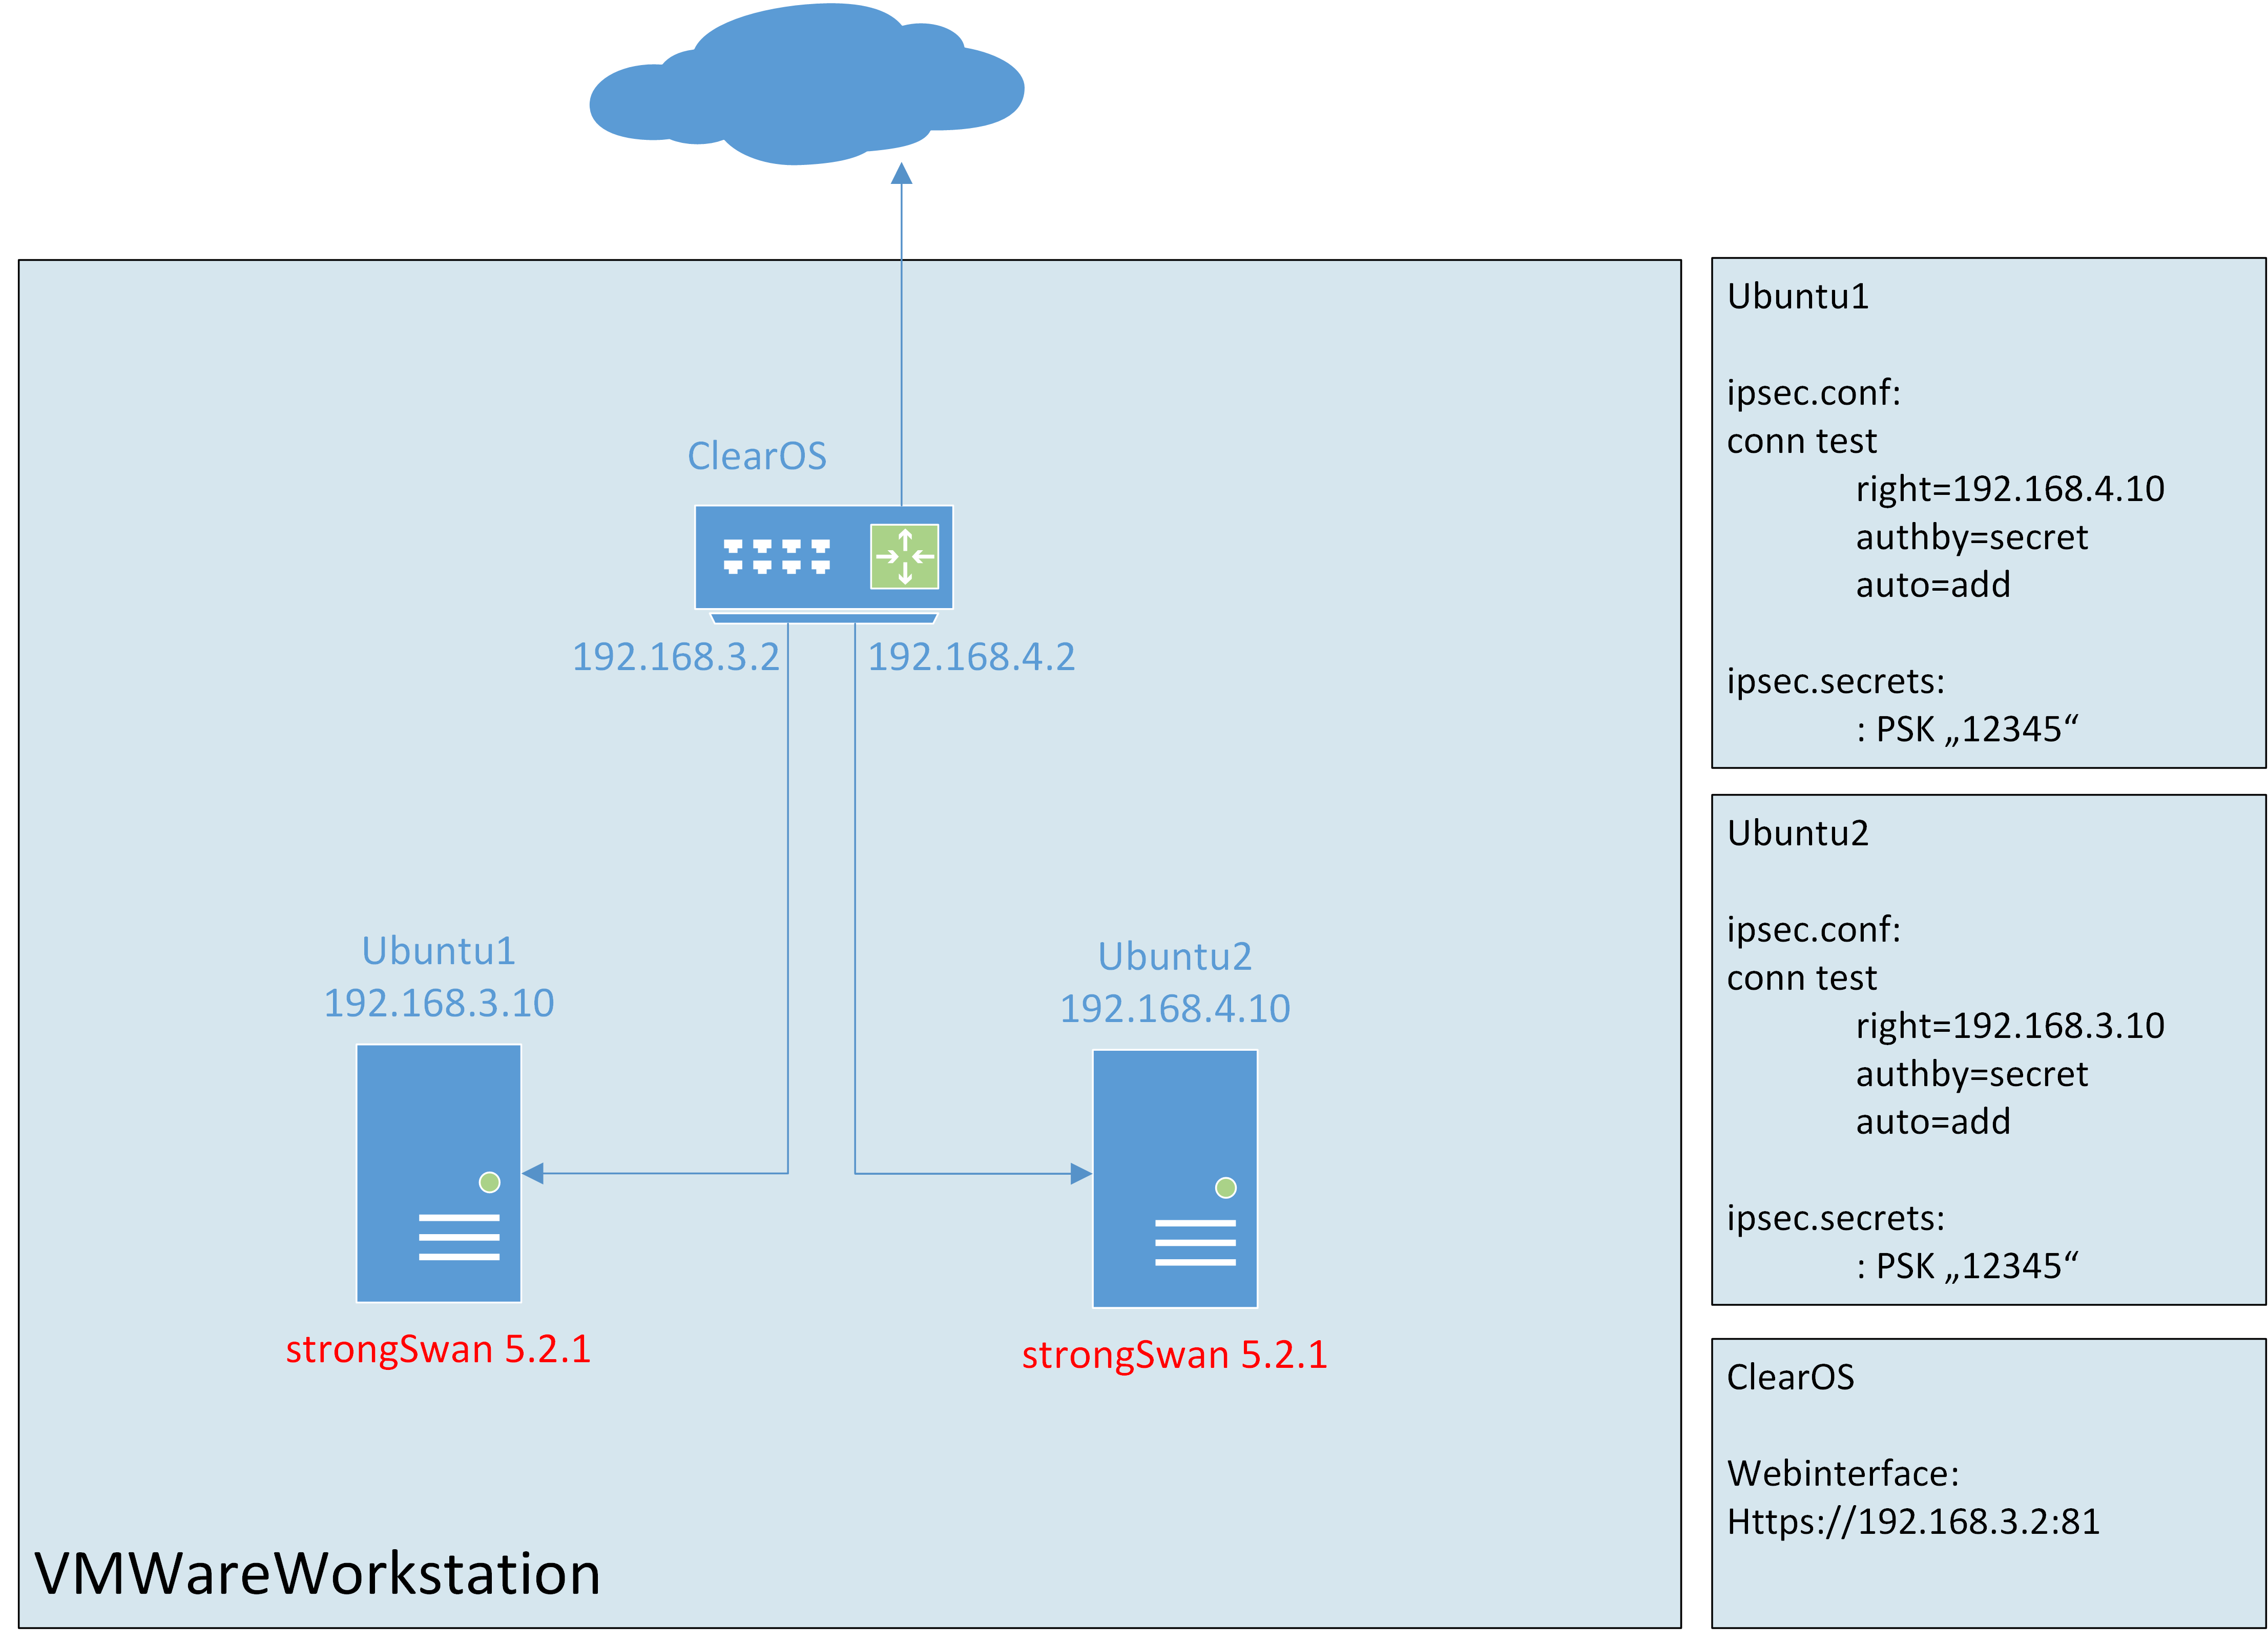
\includegraphics[width=1\textwidth]{start/img/Testumgebung.png}

\todo{Jan: Grafik anpassen}
\todo{Strongswan --> strongSwan umnennen}
\todo{Client, Server Bezeichnung entfernen}

\section{Testumgebung an der HSR}
\todo{Jan: Grafik für Rechner im SA Zimmer erstellen}
\todo{analog zu oben.}
\chapter{Testprotokoll}
\label{chap:Testprotokoll}

\section{Durchführung}
\textbf{Datum:} \\
\textbf{Ort:} \\
\textbf{Getestete Version (GitHub Hash):} \\

\section{Testfälle}

% \Square = leer, \XBox = mit X, \CheckedBox = mit Häckchen
\subsection{Allgemein}
\begin{itemize}
\item[\Square] \textbf{Kompilierung und Deployment:}\\
Das \tool lässt sich auf dem Test-System kompilieren und am erwarteten Speicherort (/opt/ipsecdiagtool/) deployen.
			   
\item[\Square] \textbf{Konfiguration finden:} \\
Das Konfigurationsfile wird am korrekten Ort (/opt/ipsecdiagtool/etc/ipsecdiagtool.conf) erstellt und kann im System gefunden werden. 
			   
\item[\Square] \textbf{Konfiguration anpassen:} \\
Das Konfigurationsfile kann verändert werden und wird beim nächsten Programmstart korrekt eingelesen.
\begin{enumerate} \itemsep1pt \parskip0pt \parsep0pt
  \item Config öffnen, AppID auf 1 setzen.
  \item Das Tool mit dem Debug-Flag starten
  \item Überprüfen ob 1 als AppID ausgegeben wird.
\end{enumerate}

\item[\Square] \textbf{Funktionalität via Help überprüfen:} \\
Das \tool soll via 'ipsecdiagtool help' gestartet werden. Alle aufgelisteten Kommandos und Beispiele sollen ausgeführt werden um zu überprüfen dass sie korrekt aufgelistet wurden.

\item[\Square] \textbf{Daemon Installieren:} \\
Das Tool lässt sich als Daemon installieren und starten.
\begin{enumerate} \itemsep1pt \parskip0pt \parsep0pt
  \item Das Tool starten via 'ipsecdiagtool install'.
  \item SysV wählen.
  \item Überprüfen ob der Daemon verfügbar ist mit 'service ipsecdiagtool start', 'service ipsecdiagtool status', 'service ipsecdiagtool stop'
\end{enumerate}

\item[\Square] \textbf{Daemon Deinstallieren:} \\
Der vom Tool installierte Daemon lässt sich wieder entfernen.
\begin{enumerate} \itemsep1pt \parskip0pt \parsep0pt
  \item Das Tool starten via 'ipsecdiagtool remove'.
  \item SysV wählen.
  \item Überprüfen ob der Daemon deinstalliert wurde mit 'service ipsecdiagtool start'. Wenn ein Fehler kommt wurde er korrekt deinstalliert.
\end{enumerate}
			   
\end{itemize}

\subsection{MTU}
\begin{itemize}
\item[\Square] \textbf{Interaktive MTU Discovery:}\\
Sicherstellen das die MTU Discovery lokal korrekt funktioniert.
\begin{enumerate} \itemsep1pt \parskip0pt \parsep0pt
  \item Bestehende Konfigurationsfiles löschen.  
  \item Das Tool als Daemon installieren 'ipsecdiagtool install' und starten 'start ipsecdiagtool'.
  \item Das Tool lokal starten via 'ipsecdiagtool i mtu'.
  \item Das Tool sollte nun die in der Konfiguration eingestellte SnapLen als MTU melden.
\end{enumerate}
			   
\item[\Square] \textbf{MTU Discovery für ein Tunnel:}\\
Das Tool soll die MTU eines echten IPSec Tunnels ermitteln.
\begin{enumerate} \itemsep1pt \parskip0pt \parsep0pt
  \item Bestehende Konfigurationsfiles neu erstellen oder anpassen so dass folgende Einstellungen konfiguriert sind: SyslogServer, SourceIP, DestinationIP. Die restlichen Einstellungen könne auf den Default Einträgen belassen werden.
  \item Das Tool an beiden Enden des Tunnels als Daemon installieren 'ipsecdiagtool install' und starten 'service ipsecdiagtool start'.
  \item Auf einer Seite des Tunnels die MTU Discovery mit dem lokalen Kommando 'ipsecdiagtool mtu' starten.
  \item Die MTU Discovery wird nun via Tunnel durchgeführt. Das erfolgreiche Resultat sollte auf dem Syslog-Server ersichtlich sein.
\end{enumerate}

\item[\Square] \textbf{MTU Discovery für mehrere Tunnels:}\\
Das Tool soll die MTU von mehreren IPSec Tunnels gleichzeitig feststellen.
\begin{enumerate} \itemsep1pt \parskip0pt \parsep0pt
  \item Bestehende Konfigurationsfiles neu erstellen oder anpassen so dass folgende Einstellungen für 2 oder mehr Tunnels konfiguriert sind: SyslogServer, SourceIP, DestinationIP. Die restlichen Einstellungen könne auf den Default Einträgen belassen werden.
  \item Das Tool an beiden Enden des Tunnels als Daemon installieren 'ipsecdiagtool install' und starten 'service ipsecdiagtool start'.
  \item Auf einer Seite des Tunnels die MTU Discovery mit dem lokalen Kommando 'ipsecdiagtool mtu' starten.
  \item Die MTU Discovery wird nun für alle Tunnels durchgeführt. Das erfolgreiche Resultat sollte auf dem Syslog-Server ersichtlich sein.
\end{enumerate}

\item[\Square] \textbf{MTU Discovery mit unterschiedlicher Anzahl Paketen:}\\
Das Tool soll die gleiche MTU mit einer unterschiedlichen Anzahl an Paketen feststellen.
\begin{enumerate} \itemsep1pt \parskip0pt \parsep0pt
  \item Bestehende Konfigurationsfiles neu erstellen oder anpassen so dass folgende Einstellungen konfiguriert sind: SyslogServer, SourceIP, DestinationIP, ConcurrentPackets. Die restlichen Einstellungen könne auf den Default Einträgen belassen werden.
  \item Das Tool an beiden Enden des Tunnels als Daemon installieren 'ipsecdiagtool install' und starten 'service ipsecdiagtool start'.
  \item Auf einer Seite des Tunnels die MTU Discovery mit dem lokalen Kommando 'ipsecdiagtool mtu' starten.
  \item Nach einem erfolgreichen Durchlauf soll der in "ConcurrentPackets" eingestellte Wert geändert werden. (z.B. in 10er Schritten erhöhen). Die jeweils festgestellte MTU soll aufgeschriben werden.
    \item Am Schluss sollen die notierten MTU Werte verglichen werden. Der Test ist erfolgreich wenn bei 5 Tests nicht mehr als eine Abweichung auftritt.
\end{enumerate}

\end{itemize}
\subsection{Packetloss}
\begin{itemize}
\item[\Square] \textbf{Interaktive Packetloss Discovery:}\\
Sicherstellen das ESP Pakete verarbeitet werden.
\begin{enumerate} \itemsep1pt \parskip0pt \parsep0pt
  \item Bestehende Konfigurationsfiles anpassen.  
  \item Das Tool als Daemon installieren 'ipsecdiagtool install' und starten 'start ipsecdiagtool'.
  \item Das Tool lokal starten via 'ipsecdiagtool i packetloss'.
  \item Das Tool sollte nun ankommende und ausgehende ESP-Packete anzeigen.
\end{enumerate}

\begin{itemize}
\item[\Square] \textbf{Packetloss via PCAP-File feststellen:}\\
Sicherstellen, ob Packete eines PCAP-Files korrekt verarbeitet und der Packetloss korrekt angezeigt wird.
\begin{enumerate} \itemsep1pt \parskip0pt \parsep0pt
  \item Bestehende Konfigurationsfiles anpassen.  
  \item Das Tool als Daemon installieren 'ipsecdiagtool install' und starten 'start ipsecdiagtool'.
  \item Das Tool lokal starten via 'ipsecdiagtool i packetloss'.
  \item Das Tool sollte nun einen Eintrag im Syslog Server erstellen mit der korrekten Meldung über den Verlust von Paketen. Gleichzeitig sollte ein CSV-File mit den Verlorenen Paketen angelegt werden.
\end{enumerate}

\begin{itemize}
\item[\Square] \textbf{Packetloss via live Capture feststellen}\\
Sicherstellen, ob Packete bei live capturing verarbeitet und der Packetloss korrekt angezeigt wird.
\begin{enumerate} \itemsep1pt \parskip0pt \parsep0pt
  \item Bestehende Konfigurationsfiles anpassen.  
  \item Das Tool als Daemon installieren 'ipsecdiagtool install' und starten 'start ipsecdiagtool'.
  \item Das Tool lokal starten via 'ipsecdiagtool i packetloss'.
  \item Das Tool sollte nun einen Eintrag im Syslog Server erstellen mit der korrekten Meldung über den Verlust von Paketen. Gleichzeitig sollte ein CSV-File mit den Verlorenen Paketen angelegt werden.
\end{enumerate}

\end{itemize}


\end{document}

%todo: abkürzungen VPS, etc. checken z.B. bei Arbeitsumegebung

% NOTE:
% Für golang ist folgendes .sty file notwendig:
% File: https://bitbucket.org/korfuri/golang-latex-listings/src/6334c5cbf471085577d7c1cfa87c29103299e37f/lstlang0.sty?at=default
% Anleitung: http://tex.stackexchange.com/questions/63496/how-to-add-go-to-the-programming-languages-list-in-lyx
% Location unter OS X: http://stackoverflow.com/questions/1390828/how-do-i-install-a-latex-sty-file-on-osx